
\chapter{Automate décrivant les polyominos inscrits dans un rectangle}
Dans ce chapitre nous allons mettre en place une structure permettant la génération et l'énumération de familles de polyominos  inscrits dans un rectangle.


 En considérant un polyomino inscrit dans un rectangle donné, ce dernier peut être décomposé comme une suite de lignes du haut vers le bas comme l'illustre  la figure \ref{Atfig1}.
\begin{figure}[!htb]
\begin{minipage}[c]{.46\linewidth}
        \centering
\end{minipage}\hfill
\begin{minipage}[c]{.23\linewidth}
        \centering
\begin{logicpuzzle}[rows=3,columns=3,color=cyan!100,width=750px,scale=0.5]
\fillcell{1}{3}
\fillcell{2}{3}
\fillcell{2}{2}
\fillcell{1}{1}
\fillcell{2}{1}
\fillcell{3}{1}
\framepuzzle[black!50]
\end{logicpuzzle}
($P$)\quad\quad\quad\quad\quad
\end{minipage}
\hfill
\begin{minipage}[c]{.32\linewidth}
 \centering
\begin{logicpuzzle}[rows=1,columns=3,color=cyan!100, width=750px,scale=0.5]
\fillcell{1}{1}
\fillcell{2}{1}
\framepuzzle[black!50]
\end{logicpuzzle}
\hfill
\begin{minipage}[c]{.95\linewidth}
 \centering
\begin{logicpuzzle}[rows=1,columns=3,color=cyan!100, width=750px,scale=0.5]
\fillcell{2}{1}
\framepuzzle[black!50]
\end{logicpuzzle}
\end{minipage}
\hfill
\begin{logicpuzzle}[rows=1,columns=3,color=cyan!100, width=750px,scale=0.5]
\fillcell{1}{1}
\fillcell{2}{1}
\fillcell{3}{1}
\framepuzzle[black!50]
\end{logicpuzzle}
\hfill
\end{minipage}
\hfill
\caption{\label{Atfig1} Décomposition de ($P$) en une suite de lignes.}
\end{figure}
Ainsi chaque ligne représente un état dans la construction dudit polyomino.
En se servant de la théorie des automates et des transducteurs, nous proposons de construire l'automate générateur de quelques familles de polyominos  inscrits dans des rectangles d'une largeur $B$ fixée, et d'une hauteur $H$ variable. Les automates que nous construisons  peuvent être plutôt vus comme des transducteurs pondérés dont les poids (coefficients de pondération ou multiplicités) sont pris dans $\mathbb{N}$ (des $\mathbb{N}$-automates) mais nous choisissons d'utiliser le terme automate puisque c'est  principalement le langage reconnu qui nous intéresse.

Dans un premier temps, nous présentons quelques généralités sur ces automates. Ensuite, nous  focalisons sur les cas $B=2$ et  $B=3$. 
\section{Généralités}
\begin{spacing}{0.30}
\subsection{État}
\end{spacing}
On considère une famille de rectangles de largeur $B$.
Pour commencer, nous représentons chaque ligne d'un rectangle de $B$ par un nombre binaire (figure \ref{Atfigb}). Chaque case occupée par une cellule sera marquée $1$ et $0$ si les cellules sont vides.

\begin{figure}[!htb]
\begin{minipage}[c]{.96\linewidth}
 \centering
\begin{minipage}[c]{.26\linewidth}
        \centering
\begin{logicpuzzle}[rows=1,columns=5,color=cyan!100,width=750px,scale=0.5]
\setrow{1}{{1},{},{},{},{}}
\fillcell{1}{1}
\fillcell{5}{1}
\end{logicpuzzle}
$1$\mbox{ }\mbox{ }$0$\mbox{ }\mbox{ }$0$\mbox{ }\mbox{ }$0$\mbox{ }\mbox{ }$1$\mbox{ }\mbox{ }\mbox{ }\mbox{ }\mbox{ }
\end{minipage}\hfill
\begin{minipage}[c]{.26\linewidth}
 \centering
\begin{logicpuzzle}[rows=1,columns=5,color=cyan!100,width=750px,scale=0.5]
\setrow{1}{{1},{},{},{},{}}
\fillcell{1}{1} 
\fillcell{3}{1} 
\end{logicpuzzle}
$1$\mbox{ }\mbox{ }$0$\mbox{ }\mbox{ }$1$\mbox{ }\mbox{ }$0$\mbox{ }\mbox{ }$0$\mbox{ }\mbox{ }\mbox{ }\mbox{ }\mbox{ }
\end{minipage}\hfill
\begin{minipage}[c]{.26\linewidth}
 \centering
 \begin{logicpuzzle}[rows=1,columns=5,color=cyan!100,width=750px,scale=0.5]
\setrow{1}{{1},{},{},{},{}}
\fillcell{1}{1} 
\fillcell{2}{1} 
\fillcell{3}{1} 
\fillcell{4}{1} 
\end{logicpuzzle}
$1$\mbox{ }\mbox{ }$1$\mbox{ }\mbox{ }$1$\mbox{ }\mbox{ }$1$\mbox{ }\mbox{ }$0$\mbox{ }\mbox{ }\mbox{ }\mbox{ }\mbox{ }
\end{minipage}
\end{minipage}
\caption{Représentation de trois lignes d'un rectangle de type  $5$ par des nombres binaires \label{Atfigb} .}
\end{figure}
Sur chaque ligne (non vide) il y a au moins une cellule et les  cellules se répartissent en sous-ensembles connexes, séparés  l'un de l'autre  par des cases vides. Pour une ligne donnée, chacun de ses sous-ensembles connexes maximaux est appelé \emph{composante connexe} de cette dernière. Deux composantes connexes disjointes sur une ligne peuvent être connectées par le haut. Pour mieux  distinguer ces composantes connexes l'une de l'autre, on propose de les numéroter de la gauche vers la droite en commençant par  $0$. 
\begin{Ex}\label{ex1}
\begin{figure}[!htb]
\begin{minipage}[c]{.16\linewidth}
        \centering
\end{minipage}
\hfill
\begin{minipage}[c]{.70\linewidth}
        \centering
\begin{logicpuzzle}[rows=1,columns=10,color=cyan!100, width=750px,scale=0.5]
\setrow{1}{{1},{},{},{},{}}
\fillcell{1}{1}
\fillcell{2}{1}
\fillcell{4}{1}
\fillcell{5}{1}
\fillcell{6}{1}
\fillcell{8}{1}
\fillcell{9}{1}
\end{logicpuzzle}
\mbox{ }\mbox{ }\mbox{ }$0$\quad \quad\quad\mbox{ }\mbox{ }$1$\quad \quad\quad\mbox{ }\mbox{ }\mbox{ }\mbox{ }$2$\quad\quad\quad\quad\quad\quad\quad\quad\quad\quad\quad\quad\quad\mbox{ }
\end{minipage}
\caption{\label{Atfig3} Les composantes connexes d'une ligne.}
\end{figure}
La ligne de la figure \ref{Atfig3} a $3$ composantes dont la première numérotée $0$ a deux cellules, la deuxième numérotée $1$ a $3$ cellules et la dernière numérotée $2$ a $2$ cellules.
\end{Ex}
\begin{Def}\label{defAt1}
Une ligne d'un rectangle de type $B$ est  une liste de $B$ éléments de $\{0,1\}$ différente de la $B$ liste constituée uniquement de $0$. C'est tout élément de $\{0,1\}^{B}$ ($\{0,1\}^{B}=\underbrace{\{0,1\}\times\{0,1\}\times...\times \{0,1\}}_{B \text{ facteurs}}$) sauf l'élément $\underbrace{00...0}_{B}.$


L'ensemble des lignes d'un rectangle de type $B$ est alors l'ensemble des $B$ listes d'éléments de $\{0,1\}$ privé de la $B$ liste constituée uniquement de $0$. 
\end{Def}
Dans la suite de ce travail on suppose que la position de chaque case  est repérée par un repère ligne d'origine $1$ c'est-à-dire que la première case est à gauche de la ligne tandis que la dernière est à la position $B$. 


Bien que du point de vue de la forme certaines lignes de rectangle puissent se ressembler, il peut arriver qu'elles ne traduisent pas les mêmes réalités.
\begin{figure}[!htb]
\begin{minipage}[c]{.16\linewidth}
        \centering
\end{minipage}
\hfill
\begin{minipage}[c]{.66\linewidth}
        \centering
\begin{logicpuzzle}[rows=5,columns=4,color=cyan!100, width=750px,scale=0.5]
\setrow{3}{{},{},}
\setrow{2}{,,{}}
\setrow{1}{{},{},{}}
\fillcell{1}{5}
\fillcell{2}{5}
\fillcell{4}{5}
\fillcell{1}{4}
\fillcell{2}{4}
\fillcell{3}{4}
\fillcell{4}{4}
\fillcell{1}{3}
\fillcell{2}{3}
\fillcell{4}{3}
\fillcell{2}{2}
\fillcell{2}{1}
\framepuzzle[black!50]
\end{logicpuzzle}
\end{minipage}
\caption{\label{Atfig4} Différence entre les lignes ayant les mêmes composantes connexes.}
\end{figure} 
Comme par exemple le cas de la figure \ref{Atfig4}, la première et la troisième ligne ont la même distribution  mais leurs composantes connexes ne sont pas liées par le haut de la même façon. Puisqu'on a convenu que la génération des polyominos se fait du haut vers le bas, si nous revenons sur la figure \ref{Atfig4} on peut  dire que les deux composantes connexes de la ligne $1$ n'ont aucune interaction entre elles par le haut. Par contre, celles de la troisième ligne sont connectées par le haut via la ligne $2$.

Ainsi pour distinguer ces cas, nous introduisons la notion de \emph{composante connexe par le haut}.

\begin{Def}\label{defAt2}
Soit $L$ une ligne d'un rectangle de largeur $B$. On dit que deux de ses composantes connexes sont connectées ou connexes par le haut s'il existe  un chemin dans le polyomino permettant de passer d'une composante connexe à l'autre par le biais des cellules des lignes en haut de $L$.

Les composantes connexes  de $L$  qui sont connectées par le haut forment alors un ensemble de composantes connexes que nous désignons par composante connexe par le haut de $L$. 
\end{Def}
\begin{Not}\label{notal1}
Soit $L$ une ligne d'un rectangle de type $B$ et $k_{1}$, $k_{2}$,..., $k_{n}$, $k_{i}, n\in\mathbb{N}$, $i=1,2,...,n$ des composantes connexes de $L$. Si $k_{1}$, $k_{2}$,..., $k_{n}$ sont connectées entre elles par le haut, la composante connexe par le haut résultante est notée 
$$\{k_{1}, k_{2},...,k_{n}\}.$$
\end{Not}
\begin{Def}\label{defAt4}
Une composante connexe par le haut d'une ligne $L$  est dite de cardinalité $n$ si elle est formée de $n$ composantes connexes de $L$.
\end{Def}
\begin{Rem}\label{remexc}
 Avec la définition \ref{defAt4}, une composante connexe non connectée par le haut à aucune autre composante connexe est aussi considérée comme une composante connexe par le haut de cardinalité $1$.
\end{Rem}
\begin{Ex}\label{ex2}
On considère la deuxième ligne de la figure \ref{AtfigN} dont les composantes connexes par le haut  sont $\{0,1\}$ de  cardinalité $2$ et
$\{2\}$  de cardinalité $1$.
\end{Ex}
\begin{figure}[!htb]
\begin{minipage}[c]{.16\linewidth}
        \centering
\end{minipage}
\hfill
\begin{minipage}[c]{.66\linewidth}
        \centering
\begin{logicpuzzle}[rows=2,columns=8,color=cyan!100, width=750px,scale=0.5]
\fillcell{1}{1}
\fillcell{4}{1}
\fillcell{5}{1}
\fillcell{7}{1}
\fillcell{8}{1}
\fillcell{4}{2}
\fillcell{3}{2}
\fillcell{2}{2}
\fillcell{1}{2}
\framepuzzle[black!50]
\end{logicpuzzle}
$0$\mbox{    }\mbox{    }\mbox{    }\mbox{    }\mbox{    }\mbox{    }\mbox{    }\mbox{    }\mbox{    }\mbox{    }$1$\mbox{    }\mbox{    }\mbox{    }\mbox{    }\mbox{    }\mbox{    }\mbox{    }\mbox{    }\mbox{    }$2$\mbox{    }\mbox{    }\mbox{    }\mbox{    }\mbox{    }\mbox{    }\mbox{    }\mbox{    }\mbox{    }\mbox{    }\mbox{    }\mbox{    }\mbox{    }\mbox{    }\mbox{    }\mbox{    }\mbox{    }\mbox{    }\mbox{    }\mbox{    }\mbox{    }\mbox{    }\mbox{    }\mbox{    }\mbox{    }\mbox{    }\mbox{    }\mbox{    }\mbox{    }\mbox{    }\mbox{    }\mbox{    }\mbox{    }\mbox{    }\mbox{    }\mbox{    }\mbox{    }\mbox{    }\mbox{    }\mbox{    }
\end{minipage}
\caption{\label{AtfigN} Exemples de composantes connexes par le haut.}
\end{figure} 
\begin{Def}\label{defAt5}
Soit 
$$E_{n} = \left\lbrace k_{1},k_{2},...,k_{n} \right\rbrace$$
l'ensemble des composantes connexes d'une ligne $L$ d'un rectangle de type $B$.  On note que l'indice $i$ de chaque élément $k_{i}$ de $E_{n}$ est le rang qu'occupe la composante connexe $k_{i}$ sur la ligne $L$ (de la gauche vers la droite).
 
On désigne par $E_{mc}$, l'ensemble composé de toutes les partitions non croisées de $E_{n}$.
Tout élément de $E_{mc}$ est appelé  partition non croisée de composantes connexes de $L$. C'est aussi une collection de composantes connexes par le haut de la ligne $L$.
\end{Def}
\begin{Ex}\label{ex3}
\begin{figure}[!htb]
\begin{minipage}[c]{.16\linewidth}
        \centering
\end{minipage}
\hfill
\begin{minipage}[c]{.7\linewidth}
        \centering
\begin{logicpuzzle}[rows=2,columns=15,color=cyan!100, width=750px,scale=0.5]
\fillcell{1}{1}
\fillcell{4}{1}
\fillcell{5}{1}
\fillcell{7}{1}
\fillcell{8}{1}
\fillcell{9}{1}
\fillcell{11}{1}
\fillcell{14}{1}
\fillcell{15}{1}
\fillcell{15}{2}
\fillcell{14}{2}
\fillcell{13}{2}
\fillcell{12}{2}
\fillcell{11}{2}
\fillcell{10}{2}
\fillcell{9}{2}
\fillcell{1}{2}
\fillcell{2}{2}
\fillcell{3}{2}
\fillcell{4}{2}
\framepuzzle[black!50]
\end{logicpuzzle}
\end{minipage}
 \caption{\label{AtfigP} Forêt de polyominos inscrite dans le rectangle $15\times 2$.}
\end{figure} 
Les ensembles $\left\lbrace \{0\}, \{ 1\}\right\rbrace $  et $\{\{0,1\},\{2,3,4\}\}$ sont respectivement des partitions non croisées de composantes connexes  de la ligne du haut et de celle du bas de la forêt de polyominos de la figure \ref{AtfigP}.
\end{Ex}
\begin{Rem}\label{remeqq}
Les éléments de $E_{n}$ sont ordonnés selon le rang qu'ils occupent sur la ligne $L$. Il y a donc une bijection entre ces derniers et leur rang. Ainsi $E_{n}$ est isomorphe à $\{1,2,...,n\}.$ Le nombre de façons de constituer des ensembles de composantes connexes par le haut de $E_{n}$ est égal au nombre de partitions non croisées de  l'ensemble $\{1,2,...,n\}.$
\end{Rem}
%\begin{Rem}\label{rem232023}
%Par définition, une ligne $L$ d'un rectangle de type $B$ a autant de partitions non croisées de composantes connexes   que  d'éléments de l'ensemble $E_{mc}$.
%\end{Rem}
\begin{Def}\label{interfm}
On considère deux lignes $L$ et $L'$, d'un rectangle de type $B$, de partitions non croisées de composantes connexes  respectives $cp_{h}$ et $cp_{h}'$. On dit que $cp_{h}$ et $cp_{h}'$ s'interceptent s'il existe au moins une composante connexe de $cp_{h}$ et une autre de $cp_{h}'$ qui se connectent. Au cas contraire on dit que $cp_{h}$ et $cp_{h}'$ ont une intersection vide.
\end{Def}
Pour alléger l'écriture, une ligne $L$ d'un rectangle de type $B$ est notée  sous la forme $L= \alpha_{1}\alpha_{2}...\alpha_{B}\in \{0,1\}^{B}$. De même le produit de deux binaires $\alpha_{i}, \alpha_{j}$ est  aussi noté $\alpha_{i}\alpha_{j}$.


Avant d'aborder la définition suivante, nous introduisons une notation utile, $deg$ (appelée degré par le haut). $deg$ est la correspondance  entre la position de chaque case de la ligne $L=\alpha_{i_{1}}\alpha_{i_{1}+1}...\alpha_{i_{1}+\mathcal{L}-1}$, de longueur $\mathcal{L}$, vue comme la ligne la plus basse d'un rectangle de type $B$ et un élément de l'alphabet $\{0,1,2,3\}$. Elle est calculée comme suit:
\begin{itemize}
\item si $\alpha_{i}=0$ alors la case correspondante n'a pas de cellule et $deg(i)=0$;

\item si $\alpha_{i}=1$ alors $deg(i)$ est le degré de la cellule située dans cette case,
\end{itemize}
où $1\leq i_{1}\leq B$ et $1\leq\mathcal{L}\leq B$.
D'une manière plus explicite et calculatoire, si nous désignons par $L'$ la ligne qui précède $L$ et par $L_{\beta}=\beta_{i_{1}}\beta_{i_{1}+1}...\beta_{i_{1}+\mathcal{L}}$  ( avec $\beta_{i_{1}}=\beta_{i_{1}+1}=...=\beta_{i_{1}+\mathcal{L}-1}=0$ si $L$ est la ligne d'un état initial) la partie de  $L'$ qui coïncide avec $L$  alors
\begin{eqnarray*}
  & &deg(i_{1})  = \alpha_{i_{1}}(\beta_{i_{1}} + \alpha_{i_{1}+1}),\\
 & &  deg(i_{1}+\mathcal{L}-1) =  \alpha_{i_{1}+\mathcal{L}-1}(\beta_{i_{1}+\mathcal{L}-1} + \alpha_{i_{1}+\mathcal{L}-2})\\
& & \textit{ et pour } i_{1}< i < i_{1}+\mathcal{L}-1, \mbox{ } 
 deg(i)  =  \alpha_{i}(\alpha_{i-1}+ \beta_{i}+\alpha_{i+1}).
 \end{eqnarray*}
 \begin{figure}[!htb]
\begin{minipage}[c]{.16\linewidth}
        \centering
\end{minipage}
\hfill
\begin{minipage}[c]{.66\linewidth}
        \centering
\begin{logicpuzzle}[rows=2,columns=8,color=cyan!100, width=750px,scale=0.5]
\fillcell{1}{2}
\fillcell{6}{1}
\fillcell{7}{1}
\fillcell{3}{1}
\fillcell{5}{1}
\fillcell{3}{2}
\fillcell{4}{2}
\fillcell{5}{2}
\fillcell{8}{2}
\fillcell{7}{2}
\fillcell{2}{2}
\framepuzzle[black!50]
\end{logicpuzzle}
\end{minipage}
\caption{\label{figdegdeg} Polyomino  inscrit dans le rectangle $8\times 2.$ }
\end{figure} 
Notons que dans la figure \ref{figdegdeg}, on a $i_{1}=3$, $\mathcal{L}=5,$ $L=10111$, $L'=11111011$ et $L_{\beta}=11101$.
\begin{Ex}\label{exdeg}
Considérons la deuxième ligne à partir du haut de la figure \ref{figdeg}.
$deg(1)=(1)(0+0)=0,\quad deg(2)=(0)(1+1+1)=0$, $deg(3)=(1)(0+1+0)=1,$ $deg(4)=(0)(1+0+1)=0$  et  $deg(5)=(1)(0+0)=0.$
\begin{figure}[!htb]
\begin{minipage}[c]{.16\linewidth}
        \centering
\end{minipage}
\hfill
\begin{minipage}[c]{.66\linewidth}
        \centering
\begin{logicpuzzle}[rows=2,columns=5,color=cyan!100, width=750px,scale=0.5]
\fillcell{1}{1}
\fillcell{3}{1}
\fillcell{5}{1}
\fillcell{3}{2}
\fillcell{2}{2}
\framepuzzle[black!50]
\end{logicpuzzle}
\end{minipage}
\caption{\label{figdeg} Calcul des valeurs  $deg$ à la ligne du bas.}
\end{figure} 
\end{Ex}
\begin{Def}\label{def20}
Un état de longueur $B$ de l'automate $\mathcal{A}_{B}$ (des polyominos contenus dans un rectangle de type $B$) est une ligne $L$ de ce rectangle, dont une case au moins est occupée par une cellule, affectée d'une  partition non croisée de composantes connexes  de $L$ et d'un mot  $m_{1}m_{2}...m_{B}$  de longueur $B$, $m_{i}\in\{0,1,2,3\}$, $i=1,2,...,B$. 
\end{Def}
\begin{Not}
Soit $L=\alpha_{1}\alpha_{2}...\alpha_{B}$ une ligne d'un rectangle de type $B$,  $\alpha_{i}\in\{0,1\}$, $\mathcal{P}_{ed}$ une partition non croisée de composantes connexes  de $L$ et $m_{1}m_{2}...m_{B}$ le mot de l'alphabet $\{0,1,2,3\}$ tel que $deg(i)=m_{i}$. Nous notons l'état $e$ de $\mathcal{A}_{B}$ de longueur $B$, généré par $L$ et $\mathcal{P}_{ed}$, par
\[e=(\alpha_{1}\alpha_{2}...\alpha_{B},m_{1}m_{2}...m_{B},\mathcal{P}_{ed}).\]

On note par $\mathcal{E}_{B}$ l'ensemble de tous les états de longueur $B$ de l'automate $\mathcal{A}_{B}$.
\end{Not}
\begin{Ex}\label{exd1} 
Les triplets $(100,000,\{\{0\}\})$, $(100,100,\{\{0\}\})$, $(111,221,\{\{0\}\})$, $(101,101,\{\{0,1\}\})$ sont des états de longueur $3$ de $\mathcal{A}_{3}$. Les états dans cet exemple correspondent respectivement du haut vers le bas aux lignes du rectangle de la  figure \ref{figetatex}.
\begin{figure}[!htb]
\begin{minipage}[c]{.16\linewidth}
        \centering
\end{minipage}
\hfill
\begin{minipage}[c]{.66\linewidth}
        \centering
\begin{logicpuzzle}[rows=4,columns=3,color=cyan!100, width=750px,scale=0.5]
\fillcell{1}{4}
\fillcell{1}{3}
\fillcell{1}{2}
\fillcell{2}{2}
\fillcell{3}{2}
\fillcell{1}{1}
\fillcell{3}{1}
\framepuzzle[black!50]
\end{logicpuzzle}
\end{minipage}
\caption{\label{figetatex} Polyomino inscrit dans le rectangle  $3\times 4$.}
\end{figure} 
\end{Ex}
Nous définissons dans $\mathcal{E}_{B}$ une relation $\mathcal{R}_{B}$. Étant donné $e, e'\in \mathcal{E}_{B}$, 
\begin{eqnarray}\label{rel}
& & e \mathcal{R}_{B} e' \textit{ si et seulement si } e \textit{ et } e' \textit{  ont la même ligne}\\ \nonumber
& &\textit{ et la même partition non croisée de composantes connexes}
\end{eqnarray}
\begin{Prop}\label{prop20}
$\mathcal{R}_{B}$ est une relation d'équivalence.
\end{Prop}
\begin{Pre}
En effet, 
\begin{itemize}
\item $\mathcal{R}_{B}$ est réflexive  car tout état $e=(\alpha_{1}\alpha_{2}...\alpha_{B},m_{1}m_{2}...m_{B},\mathcal{P}_{ed}) $ de $\mathcal{E}_{B}$ est en relation avec lui même.

\item Soit $e=(\alpha_{1}\alpha_{2}...\alpha_{B},m_{1}m_{2}...m_{B},\mathcal{P}_{ed})$ et $e'=(\alpha'_{1}\alpha'_{2}...\alpha'_{B},m'_{1}m'_{2}...m'_{B},\mathcal{P}'_{ed})$ tels que $e\mathcal{R}_{B} e'$. On a  $\alpha_{1}\alpha_{2}...\alpha_{B}=\alpha'_{1}\alpha'_{2}...\alpha'_{B}$ et $\mathcal{P}_{ed}= \mathcal{P}'_{ed}$ donc $e'\mathcal{R}_{B} e$. $\mathcal{R}_{B}$ est alors symétrique.

\item Soit $e=(\alpha_{1}\alpha_{2}...\alpha_{B},m_{1}m_{2}...m_{B},\mathcal{P}_{ed})$ et $e'=(\alpha'_{1}\alpha'_{2}...\alpha'_{B},m'_{1}m'_{2}...m'_{B},\mathcal{P}'_{ed})$ et $e''=(\alpha''_{1}\alpha''_{2}...\alpha''_{B},m''_{1}m''_{2}...m''_{B},\mathcal{P}''_{ed})$ tels que $e\mathcal{R}_{B} e'$ et  $e'\mathcal{R}_{B} e''$. On a alors $\alpha_{1}\alpha_{2}...\alpha_{B}=\alpha'_{1}\alpha'_{2}...\alpha'_{B}, \mathcal{P}_{ed}=\mathcal{P}'_{ed}$ d'une part et  $\alpha'_{1}\alpha'_{2}...\alpha'_{B}=\alpha''_{1}\alpha''_{2}...\alpha''_{B}, \mathcal{P}'_{ed}=\mathcal{P}''_{ed}$ d'autre part. On en déduit que $\alpha_{1}\alpha_{2}...\alpha_{B}=\alpha''_{1}\alpha''_{2}...\alpha''_{B}, \mathcal{P}_{ed}=\mathcal{P}''_{ed}$, d'où $e \mathcal{R}_{B} e''$. Ce qui confirme la transitivité de $\mathcal{R}_{B}$.
\end{itemize} 
Le quotient  $\frac{\mathcal{E}_{B}}{\mathcal{R}_{B}}$ est noté $\mathbb{E}_{B}$.
\end{Pre}
\begin{Def}\label{defAt6}

Un élément de  $\mathbb{E}_{B}$ est appelé classe d'états ou état fondamental de longueur $B$ de $\mathcal{A}_{B}$.
\end{Def}
\begin{Rem}\label{remd1}
Les mots de l'alphabet $\{0,1,2,3\}$, utilisés dans la définition des états  de l'automate $\mathcal{A}_{B}$, facilitent le calcul du nombre de feuilles des polyominos inscrits dans un rectangle de type $B$. Ainsi si l'on ne tenait compte que des paramètres aire et périmètre, un état de $\mathcal{A}_{B}$ serait un couple de ligne et d'une partition non croisée de composantes connexes. C'est ce qui justifie, d'ailleurs, le terme état fondamental utilisé pour désigner une classe d'états de $\mathcal{A}_{B}$. Dans ce cas seul  $\mathbb{E}_{B}$ et $\mathcal{E}_{B}$  serait pertinent. 
%Une classe d'états de $\mathcal{A}_{B}$ sera aussi souvent représentée par la lettre $e$ comme le cas des états, mais à la seule différence que $e$ en tant que classe d'états correspond au couple $(\alpha_{1}\alpha_{2}...\alpha_{B},\mathcal{P}_{ed})$. De plus, dès que le mot de l'alphabet $\{0,1,2,3\}$ associé à un état n'est pas nécessaire pour expliquer une situation, nous utilisons la forme correspondante à un état fondamental (un couple formé d'une ligne et d'une partition non croisée de composantes connexes  ) au lieu de la forme d'état (un triplet  formé d'une ligne, d'un mot de l'alphabet $\{0,1,2,3\}$  et d'une partition non croisée de composantes connexes  par le haut).
\end{Rem}
\begin{Rem}\label{rem1}
Soit $L$ une ligne possible, de longueur $B$, d'un rectangle de type $B$, pouvant être la première ligne ou une ligne précédée par d'autres.
 $L$ génère autant d'états  fondamentaux de longueur $B$ que de partitions non croisées de composantes connexes.
\end{Rem}
\begin{Ex}\label{exrec}
\begin{figure}[!htb]
\begin{minipage}[c]{.16\linewidth}
        \centering
\end{minipage}
\hfill
\begin{minipage}[c]{.66\linewidth}
        \centering
\begin{logicpuzzle}[rows=1,columns=10,color=cyan!100, width=750px,scale=0.5]
\fillcell{1}{1}
\fillcell{2}{1}
\fillcell{4}{1}
\fillcell{5}{1}
\fillcell{6}{1}
\fillcell{7}{1}
\fillcell{8}{1}
\fillcell{10}{1}
\framepuzzle[black!50]
\end{logicpuzzle}
\end{minipage}
\caption{\label{figclass} Ligne d'un rectangle de type $10$.}
\end{figure} 
La ligne de la figure \ref{figclass}, $1101111101$, génère $5$ partitions non croisées de composantes connexes  notamment $$\{\{0\},\{1\},\{2\}\}, \{\{0,1\},\{2\}\}, \{\{0\},\{1,2\}\}, \{\{0,2\},\{1\}\} \textit{ et }\{\{0,1,2\}\}.$$ Pour obtenir l'état fondamental correspondant à chaque partition non croisée de composantes connexes  , il suffit de former le couple composé de la ligne et de cette dernière comme par exemple $(1101111101,\{\{0,2\},\{1\}\})$.
\end{Ex}
\begin{Rem}\label{reg}
\begin{spacing}{0.27}
\section*{Règle sur le choix de la longueur d'un état}
\end{spacing}
Il peut arriver dans certains cas qu'un polyomino inscrit, à une étape donnée, évolue  uniquement suivant une bande  de largeur $B'$, $B'< B$, sans  déborder jusqu'à la base du  rectangle (voir figure \ref{ATfig5}).
\begin{figure}[!htb]
\begin{minipage}[c]{.30\linewidth}
        \centering
\end{minipage}
\hfill
\begin{minipage}[c]{.95\linewidth}
\begin{minipage}[c]{.30\linewidth}
        \centering
\begin{logicpuzzle}[rows=6,columns=7,color=cyan!100,width=750px,scale=0.5]
\setrow{3}{{},{},}
\setrow{2}{,,{}}
\setrow{1}{{},{},{}}
\fillcell{1}{6}
\fillcell{2}{6}
\fillcell{7}{6}
\fillcell{1}{5}
\fillcell{2}{5}
\fillcell{3}{5}
\fillcell{4}{5}
\fillcell{5}{5}
\fillcell{6}{5}
\fillcell{7}{5}
\fillcell{1}{4}
\fillcell{2}{4}
\fillcell{3}{4}
\fillcell{1}{3}
\fillcell{2}{3}
\fillcell{3}{3}
\fillcell{1}{2}
\fillcell{2}{2}
\fillcell{1}{1}
\framepuzzle[black!50]
\end{logicpuzzle}
\end{minipage}
\hfill
\begin{minipage}[c]{.36\linewidth}
        \centering
\begin{logicpuzzle}[rows=6,columns=7,color=cyan!100, width=750px,scale=0.5]
\setrow{3}{{},{},}
\setrow{2}{,,{}}
\setrow{1}{{},{},{}}
\fillcell{1}{6}
\fillcell{2}{6}
\fillcell{3}{6}
\fillcell{4}{6}
\fillcell{5}{6}
\fillcell{6}{6}
\fillcell{7}{6}
\fillcell{3}{5}
\fillcell{4}{5}
\fillcell{5}{5}
\fillcell{3}{4}
\fillcell{4}{4}
\fillcell{5}{4}
\fillcell{3}{3}
\fillcell{4}{3}
\fillcell{5}{3}
\fillcell{4}{2}
\fillcell{5}{2}
\fillcell{4}{1}
\fillcell{5}{1}
\framepuzzle[black!50]
\end{logicpuzzle}
\end{minipage}
\end{minipage}
 \caption{\label{ATfig5} Polyominos inscrits dans le rectangle de type $7$ de hauteur $6$.}
\end{figure} 

 Dans ce cas, la partie du polyomino inscrite dans cette bande peut être vue comme un polyomino inscrit dans un rectangle de largeur $B'$.  Ainsi pour décrire cette partie du polyomino, on impose l'utilisation d'un état de longueur égale à la longueur d'une telle bande. De plus au fur et à mesure que la longueur de la bande diminue, on réajuste la longueur d'état par rapport à la nouvelle bande.
\end{Rem} 
 Ainsi, les états de l'automate $\mathcal{A}_{B'}$  sont aussi des états  de l'automate $\mathcal{A}_{B}$.
\begin{Rem}\label{remd2}
Les cases des lignes de tout état $e$ de $\mathcal{A}_{B}$ sont toujours étiquetées dans un repère universel, celui correspondant aux états de longueur $B$. Ainsi, si nous avons un état de longueur $B'\leq B$, si sa première case est située à la position $i_{1}$, $i_{1}\geq 1$, alors la dernière sera donc à la position $B'+i_{1}-1$.
\end{Rem}
\begin{Def}\label{defAt7}
Soit $\mathbf{E}_{B}$ l'ensemble de tous les états  de $\mathcal{A}_{B}$.
Alors 

$$\mathbf{E}_{B}= \mathcal{E}_{B}\cup \mathcal{E}_{B-1}\cup...\cup \mathcal{E}_{1}.$$

En notant par $\mathfrak{E}_{B}$ l'ensemble de tous les états fondamentaux de $\mathcal{A}_{B}$, on a

$$\mathfrak{E}_{B}=\mathbb{E}_{B}\cup\mathbb{E}_{B-1}\cup ... \cup \mathbb{E}_{1}. $$
\end{Def}

\begin{Ex}\label{ex4}
Nous considérons le cas $B=3$.

Les lignes possibles d'un rectangle de type $3$ sont $L_{1}=100$, $L_{2}=010$, $L_{3}=001$, $L_{4}=110$, $L_{5}=101$, $L_{6}=011$ et $L_{7}=111$. Chacune des lignes précédentes a une seule composante connexe sauf la ligne $L_{5}$ qui en a deux. Les partitions non croisées de composantes connexes  de $L_{5}$ sont donc $\{\{0\},\{1\}\}$  et $\{\{0,1\}\}$.

On a 
$$\mathbb{E}_{3}=\{ (100,\lbrace\lbrace 0\rbrace\rbrace),(010,\lbrace\lbrace 0\rbrace\rbrace),(001,\lbrace\lbrace 0\rbrace\rbrace), (110,\lbrace\lbrace 0\rbrace\rbrace),(101,\lbrace\lbrace 0\rbrace,\lbrace 1\rbrace\rbrace),$$
$$(101,\lbrace\lbrace 0,1\rbrace\rbrace),(011,\lbrace\lbrace 0\rbrace\rbrace),(111,\lbrace\lbrace 0\rbrace\rbrace) \}.$$

De même 
$$\mathbb{E}_{2}=\left\lbrace (10,\lbrace \lbrace 0\rbrace\rbrace),(01,\lbrace\lbrace 0\rbrace\rbrace),(11,\lbrace\lbrace 0\rbrace\rbrace) \right\rbrace .$$ Et
$$\mathbb{E}_{1}= \left\lbrace  (1,\lbrace\lbrace 0\rbrace\rbrace)\right\rbrace .$$

On obtient 
$$\mathfrak{E}_{3}=\mathbb{E}_{3}\cup\mathbb{E}_{2}\cup\mathbb{E}_{1}. $$
\end{Ex}
\begin{Rem}\label{rem4}
 Pour éviter de refaire certains calculs, lorsqu'il n'y a pas d'ambiguïté, nous confondons les termes état et état fondamental. Lorsque  nécessaire nous préciserons s'il s'agit d'une classe d'états. Un état est donc souvent représenté sous forme de sa classe à chaque fois que les opérations  associées ne nécessitent pas d'autres informations à part celles données par sa classe.

\end{Rem}
Par la définition d'un état de l'automate  $\mathcal{A}_{B}$, si l'on devait parler d'état initial  de cet automate cela reviendrait à parler d'un de ses états dont la ligne est l'une des premières lignes possibles d'un rectangle de type $B$. Or aucune  composante connexe d'une première ligne d'un tel rectangle n'est connectée à une autre par le haut. De plus si l'on prenait  un état de longueur $\mathcal{L}$ inférieure à $B$ comme  initial alors tous les polyominos commençant par cet état ne seraient étendues que dans la bande de largeur  $\mathcal{L}$ et non $B$. Dans ce cas, l'automate $\mathcal{A}_{\mathcal{L}}$ serait  l’automate idéal pour décrire ces polyominos. On a alors la définition suivante.
\begin{Def}\label{defAt8}
Soit $e=(\alpha_{1}\alpha_{2}...\alpha_{B},m_{1}m_{2}...m_{B},\mathcal{P}_{ed})$ un état  de $\mathcal{A}_{B}$ de longueur $B$. 

Si $B=1$, $\alpha_{1}=1$ et $m_{1}=0$ alors $e$ est le seul état initial de $\mathcal{A}_{1}$. 

Si $B\geq 2$  $e$ est dit état initial de $\mathcal{A}_{B}$ si et seulement s'il vérifie les deux conditions suivantes:
\begin{itemize}
 \item[(i)] toutes ses composantes connexes par le haut  sont de cardinalité $1$ (c'est-à-dire qu'aucune composante connexe de la ligne de $e$ n'est connectée à une autre),  \item[(ii)]$m_{1}=\alpha_{1}\alpha_{2}$ , $m_{B}=\alpha_{B-1}\alpha_{B}$ et pour $2\leq i\leq B-1$, $m_{i}=\alpha_{i}(\alpha_{i-1}+\alpha_{i+1}).$
\end{itemize}
\end{Def}
Pour définir les états finaux de l'automate $\mathcal{A}_{B}$ nous nous basons sur la connexité des cellules des lignes précédentes jusqu'à la dernière ligne et aussi nous cherchons à garantir l'inscriptibilité de tous polyominos dont la dernière ligne est une ligne d'un de ces états. Pour des raisons de connexité, la partition non croisée de composantes connexes qui  est associées à un état final doit être de cardinalité $1$. 
\begin{Def}\label{defAt9}
Soit $e=(\alpha_{i_{1}}\alpha_{i_{1}+1}...\alpha_{\mathcal{L}+i_{1}-1},m_{i_{1}}m_{i_{1}+1}...m_{\mathcal{L}+i_{1}-1},\mathcal{P}_{ed})$  un état de longueur $\mathcal{L}$ de $\mathcal{A}_{B}$. 

 Si $\mathcal{L}=1$, $e$ est un état final de $\mathcal{A}_{B}$ si $\alpha_{i_{1}}=1$ et $m_{i_{1}}=1$.
 
Si $\mathcal{L}\geq 2$, $e$ est dit état final de $\mathcal{A}_{B}$ si et seulement s'il vérifie les conditions ci-dessous:
\begin{itemize}
 \item[(i)]$\mathcal{P}_{ed}$ est  constituée d'une seule composante connexe par le haut (c'est-à-dire que toutes les composantes connexes de la ligne de $e$ forment un ensemble connexe), 
 \item[(ii)]$\alpha_{i_{1}}=\alpha_{\mathcal{L}+i_{1}-1}=1$.
% \item[(iii)] il existe au moins une case $i_{0}$, $i_{1}\leq i_{0}\leq \mathcal{L}+i_{1}-1$ telle que $\alpha_{i_{0}}\neq 0$ et 
%\begin{itemize}
 %\item si $i_{0}=i_{1}$ alors $m_{i_{1}}> \alpha_{i_{1}+1} $
 %\item si $i_{0}=\mathcal{L}+i_{1}-1$ alors $m_{\mathcal{L}+i_{1}-1}> \alpha_{\mathcal{L}+i_{1}-2}$
% \item si $i_{1}<i_{0}<\mathcal{L}+i_{1}-1$ alors $m_{i_{0}}>\alpha_{i_{0}-1}+\alpha_{i_{0}+1}$.
%\end{itemize}
\end{itemize}
\end{Def}
Les définitions \ref{defAt8} et \ref{defAt9} peuvent être vues aussi comme des propositions mais nous choisissons d'utiliser le terme définition parce que c'est notre première fois d'aborder, dans ce mémoire,  les informations qui s'y trouvent.

%Les raisons du choix des états initiaux ont été évoquées
%\begin{Rem}\label{rem2}
%À part l'automate $\mathcal{A}_{1}$, l'automate $\mathcal{A}_{B}$, $B>1$, est  non déterministe, car il a plusieurs états initiaux. 
%\end{Rem}
\begin{Lem}\label{lem2}
Le nombre maximum de composantes connexes sur une ligne d'un rectangle de type $B$ est 
$$\left\lfloor \dfrac{B+1}{2} \right\rfloor .$$
\end{Lem}
\begin{Pre}
Le  nombre maximal de composantes connexes qu'on peut avoir sur une ligne d'un rectangle de type $B$ est le nombre maximal de ses composantes connexes à une seule cellule. Il s'agit dans ce cas d'une alternance de cases occupées et non occupées comme le cas de la figure \ref{alt1}.  Ce nombre correspond au nombre de cases vides ($\frac{B}{2}$) si $B$ est pair (c'est-à-dire la moitié des cases sur cette ligne) et au nombre de cases vides plus $1$ ($\frac{B+1}{2}$) si $B$ est impair (car il y a des cellules aux deux extrémités de la ligne). Dans les deux cas, ce nombre est exactement  $$\left\lfloor \dfrac{B+1}{2} \right\rfloor .$$
\end{Pre}
\begin{figure}[!htb]
\begin{minipage}[c]{.46\linewidth}
        \centering
\begin{logicpuzzle}[rows=1,columns=11,color=cyan!100, width=750px,scale=0.5]
\fillcell{1}{1}
\fillcell{3}{1}
\fillcell{5}{1}
\fillcell{7}{1}
\fillcell{9}{1}
\fillcell{11}{1}
\framepuzzle[black!50]
\end{logicpuzzle}
\end{minipage}
\hfill
\begin{minipage}[c]{.46\linewidth}
        \centering
\begin{logicpuzzle}[rows=1,columns=10,color=cyan!100, width=750px,scale=0.5]
\fillcell{1}{1}
\fillcell{3}{1}
\fillcell{5}{1}
\fillcell{7}{1}
\fillcell{9}{1}
\framepuzzle[black!50]
\end{logicpuzzle}
\end{minipage}
 \caption{\label{alt1} Forêts de polyominos lignes de longueurs $11$ et $10$ ayant respectivement $6$ et $5$ composantes connexes.}
\end{figure} 

\begin{Ex}\label{ex11}
Une ligne d'un rectangle de type $3$ ou de type $4$ possède au moins une composante connexe et au plus $2$ composantes connexes.
Une ligne d'un rectangle de type  $5$ ou de type  $6$ possède au moins une composante connexe et au plus $3$ composantes connexes.
\end{Ex}
\begin{Def}\label{def42023}
Soit $e$ un état de $\mathcal{A}_{B}$ de ligne $L$.

 L'aire et le périmètre de $e$ sont respectivement l'aire et le périmètre de la forêt de polyominos ligne décrite par la ligne $L$.
 
Toute case $i$ de la ligne $L$ de  $e$ telle que $deg(i)=1$ est une feuille de $e$.
\end{Def}
\begin{Prop}\label{prop12}
Soit $e$ un état d'aire $a$, de périmètre $p$ et de ligne $L$. 

Le nombre $n_{c}$ de composantes connexes sur la ligne $L$ est 

\begin{eqnarray}\label{for8}
 n_{c} & = & \frac{p-2a}{2}.
\end{eqnarray}
\end{Prop}
\begin{Pre}
La formule \ref{for8} s'explique d'une part par le fait qu'une cellule a pour aire et périmètre respectivement $1$ et $4$. Ainsi, la ligne $L$ n'a que $a$ cellules. D'autre part,  le périmètre d'une composante connexe se calcule comme étant la somme des côtés nord et sud de chaque cellule à laquelle s'ajoute le côté \emph{est} de la première cellule de la composante  connexe et le côté \emph{ouest} de sa dernière cellule. c'est-à-dire que si une composante connexe $c_{1}$ possède $a_{c_{1}}$ cellules alors son périmètre $p_{c_{1}}$ est 
$$p_{c_{1}} = 2(a_{c_{1}} + 1).$$  Si la ligne possède $n$ composantes $c_{1}, c_{2},..., c_{n} $ alors on a 
\begin{eqnarray*}
p &= & p_{c_{1}} +  p_{c_{2}} + ... + p_{c_{n}}\\
& = & 2(a_{c_{1}} + 1) + 2(a_{c_{2}} + 1) +...+ 2(a_{c_{n}} + 1)\\
&=& 2(a_{c_{1}}+ a_{c_{2}} +...+a_{c_{n}}) + 2n_{c}\\
&=& 2a+2n_{c}.
\end{eqnarray*} 
Et on a  enfin
\begin{eqnarray*}
n_{c} & = & \frac{p-2a}{2}.
\end{eqnarray*}
\end{Pre}
\begin{Ex}\label{ex13}
L'état  représenté par la deuxième ligne de la figure \ref{AtfigP}  possède $9$ cellules regroupées en $5$ composantes connexes et de périmètre $28$. Nous avons effectivement $5=\frac{10}{2}=\frac{28-18}{2}.$
\end{Ex}

On a donc la proposition suivante.
\begin{Prop}\label{prop11}
Soit $B$ un entier naturel non nul. Chaque rectangle de type $B$  a au total $2^{B}-1$ lignes possibles de longueur $B$ et chaque ligne $L_{i}$ de ce dernier ayant $n_{i}$ composantes connexes, $1\leq i\leq 2^{B}-1$,
génère au total $C_{n_{i}}$ états fondamentaux, où
\begin{eqnarray}\label{for5}
 C_{n_{i}} &=& \dfrac{(2n_{i})!}{n_{i}!(n_{i}+1)!},  
\end{eqnarray}
De plus le nombre total, $N_{B}$, d'états fondamentaux de longueur $B$ de $\mathcal{A}_{B}$ est 
\begin{eqnarray}\label{for6}
N_{B} & = & \sum_{i=1}^{2^{B}-1}C_{n_{i}}.
\end{eqnarray}
En notant par $\mathcal{N}_{B}$ le nombre total d'états fondamentaux de $\mathcal{A}_{B}$, on a 
\begin{eqnarray}\label{for7}
\mathcal{N}_{B} & = & N_{B} + N_{B-1}+...+N_{2} + N_{1} \textit{  i.e.  } \mathcal{N}_{B} = N_{B} + \mathcal{N}_{B-1}.
\end{eqnarray}
\end{Prop}
\begin{Pre}
Comme toute ligne de longueur $B$ d'un rectangle de type $B$ est un élément de $\{0,1\}^{B}$, sauf la ligne dépourvue de cellule, on a effectivement au total $2^{B}-1$ lignes. 

Par ailleurs, le nombre d'états fondamentaux générés par $L_{i}$ est  le nombre de partitions non croisées de composantes connexes  générées par ladite ligne et, d'après le théorème \ref{cat}, et la définition  d'une partition non croisée de composantes connexes  , ce nombre correspond donc au nombre de Catalan $C_{n_{i}}$ relatif  à  l'ensemble $\{1,2,...,n_{i}\}$ qui est égal à $$ \dfrac{(2n_{i})!}{n_{i}!(n_{i}+1)!}. $$
Ainsi, pour les  $2^{B}-1$ lignes possibles, le nombre $N_{B}$ d'états fondamentaux de longueur $B$ est égal à
$$\sum_{i=1}^{ 2^{B}-1}C_{n_{i}}.$$
Étant donné que tous les états de longueurs inférieures à $B$ sont aussi des états de $\mathcal{A}_{B}$, on a $\mathcal{N}_{B}  =  N_{B} + N_{B-1}+...+N_{2} + N_{1}$.
\end{Pre}
\begin{Ex}\label{ex12}
Nous calculons manuellement le nombre d'états fondamentaux de $\mathcal{A}_{B}$ pour $B=2,3,4$ et $5$, une application des formules données dans les propositions précédentes.
\begin{itemize}
\item[(i)] $\mathcal{N}_{2} = N_{2} +N_{1}$. $N_{1}$ vaut $1$. Chaque ligne d'un rectangle de type $2$ ne peut qu'avoir qu'une seule composante. Ainsi, $N_{2} = 2^{2}-1=3$. On conclut donc que $\mathcal{N}_{2} =4.$
\item[(ii)] $\mathcal{N}_{3} = N_{3} + \mathcal{N}_{2}$. $6$ lignes des rectangles de type $3$, notamment $$100, 010, 001, 110, 011, 111, $$ n'ont qu'une seule composante. Par contre une seule ligne, $101$, a deux composantes connexes. On a pour cette ligne 
\begin{eqnarray*}
C_{2} & = & \dfrac{4!}{2!3!} =  \dfrac{24}{12} =  2.
\end{eqnarray*}
Ainsi, cette ligne génère deux états. On a donc $N_{3}= 1+1+1+1+1+1 +2=8.$ Ce qui nous donne $\mathcal{N}_{3}= 8 +4 =12.$
\item[(iii)] $\mathcal{N}_{4} = N_{4} + \mathcal{N}_{3}$. D'après le Lemme \ref{lem2} sur une ligne d'un rectangle de type $4$ on a une ou deux composantes connexes. Cinq lignes ont deux composantes connexes, notamment les lignes $$1001, 0101, 1010, 1101 \textit{  et } 1011 $$  dont chacune génère  deux états.
\begin{eqnarray*}
N_{4} & = & 1+1+1+1+1+1+1+1+1+1+2+2+2+2+2=20.
\end{eqnarray*}
On a alors
\begin{eqnarray*}
 \mathcal{N}_{4} & = & 20 + 12= 32.
\end{eqnarray*}
\item[(iv)] $\mathcal{N}_{5} =N_{5} + \mathcal{N}_{4}$. Le lemme \ref{lem2} nous permet d'affirmer qu'une ligne d'un rectangle  de type $5$ ne peut qu'avoir qu'une, deux ou trois composantes connexes. Nous avons quinze lignes à deux composantes connexes qui sont les lignes
\begin{eqnarray*}
& & 10001, 10100, 10010, 01010, 01001, 00101, 10111, 11101, 11001,\\
& &11010, 01101, 10011, 10110, 01011 \textit{ et } 11011
\end{eqnarray*}
qui génère chacune deux états.
La seule ligne à trois composantes est la ligne $10101$ qui génère $C_{3}$ états avec
\begin{eqnarray*}
C_{3}=\dfrac{6!}{3!4!}  = 5.
\end{eqnarray*} On déduit
\begin{eqnarray*}
N_{5} & = &  1\times 15 + 2\times 15 + 5= 50
\end{eqnarray*}
\begin{eqnarray*}
\mathcal{N}_{5} & = & 50 +32 =82.
\end{eqnarray*}
\end{itemize}
\end{Ex}
Sur la base des formules établies dans cette section, nous écrivons un programme qui calcule le nombre d'états fondamentaux pour $B$ quelconques. Nous listons ainsi la suite $\mathcal{N}_{B}$ des nombres d'états fondamentaux  pour  $1\leq B\leq 15$:

$1$, $4$, $12$, $32$, $82$, $208$, $7$, $530$, $1364$, $3551$, $9348$
 $24858$, $66692$, $179902$, $484128$, $1285405$.

Les termes $\mathcal{N}_{1}$, $\mathcal{N}_{2}$, $\mathcal{N}_{3}$, $\mathcal{N}_{4}$, $\mathcal{N}_{5}$, $\mathcal{N}_{6}$  de cette suite sont respectivement égaux aux termes $a_{4}$, $a_{5}$, $a_{6}$, $a_{7}$, $a_{8}$ et $a_{9}$ de la suite, $a_{B}$, numéro $A135248$ de \emph{OEIS}. C'est-à-dire $\mathcal{N}_{B}=a_{B+3}$ pour $1\leq B\leq 6$. Mais à partir de $B=7$ nous n'avons plus l'égalité $\mathcal{N}_{B}=a_{B+3}$. 
\begin{spacing}{0.30}
\subsection{L'alphabet et les transitions d'états}
\end{spacing}
Dans cette sous-section, nous définissons l'alphabet associé à l'automate $\mathcal{A}_{B}$ puis  introduisons la notion de transition d'un état à l'autre. Pour un polyomino donné, $P_{B,H}$ inscrit dans un rectangle de largeur $B$ et de hauteur $H$, nous nous intéressons à son aire, son périmètre, sa hauteur et son nombre de feuilles. Les variables $w$, $x$, $y$ et $z$ sont utilisées pour compter respectivement l'aire, le périmètre, la hauteur et le nombre de feuilles de $P_{B,H}$.

 Ainsi nous désignons par
$$ \Sigma = \{w,x,y,z,z^{-1}\}$$ l'alphabet de l'automate $\mathcal{A}_{B}$.
Nous associons à $\Sigma^{*}$ l'application  suivante:
\begin{eqnarray}
F_{L}: \mathbb{N}Rat\Sigma^{*} & \longrightarrow & \mathbb{M}_{L}\nonumber\\
 m:&\longmapsto & \lambda w^{a}x^{p}y^{h}z^{f} \text{ et  si }m_{1}, m_{2}\in \mathbb{N}Rat\Sigma^{*},\\
 F_{L}(m_{1}+m_{2})&=& F_{L}(m_{1})+F_{L}(m_{2})
\end{eqnarray}
où $\mathbb{M}_{L}$ désigne l'ensemble des monômes de Laurent à quatre variables ($w,x,y,z$). Dans l'expression $\lambda w^{a}x^{p}y^{h}z^{f}$, $\lambda$ est la multiplicité du mot qui a $a$ symboles $w$, $p$ symboles $x$, $h$ symboles $y$ et $f$ le nombre du symbole $z$ moins celui du symbole $z^{-1}$ dans le mot $m$. 
\begin{Ex}\label{FL}
Soit $m=2wxwyzwz^{-1}wz^{-1}$ alors $F_{L}(m)=2w^{4}xyz^{-1}$.
\end{Ex}
Par la suite, tout mot $m$ est représenté par son image par $F_{L}$.
\begin{Def}\label{defAt10}
Une transition élémentaire $t_{i,j}$ d'un état $e_{i}$ à un état $e_{j}$ est donnée par un monôme de Laurent
$$t_{i,j}= \lambda w^{a}x^{p}yz^{f}, $$
où $a,p$ sont des entiers naturels et $f$ est un entier relatif désignant respectivement les contributions d'aire, du périmètre, de hauteur et du gain ou de la perte de feuilles lors du passage de la ligne de $e_{i}$ à la ligne de $e_{j}$ et $\lambda\in \{0,1\}$.
\end{Def}
Il peut y avoir plusieurs façons de connecter l'état $e_{j}$ à l'état $e_{i}$ (chacune d'elles est appelée \emph{décalage} de $e_{j}$ par rapport à $e_{i}$  et noté $d_{i,j}$) comme le suggère l'exemple \ref{ex10}. Chaque décalage  $d_{i,j}$ correspond à une transition élémentaire $t_{i,j}$. Lorsqu'un décalage est possible (ou admissible) $\lambda=1$ et $0$ sinon. Dans le cas où $\lambda=0$ on dit aussi que la transition élémentaire, $t_{i,j}$  associée à $d_{i,j}$ est impossible.

 Soit $n$ un entier naturel correspondant au nombre de décalages de  $e_{j}$ par rapport à $e_{i}$. Les $n$ transitions élémentaires de $e_{i}$ à $e_{j}$ correspondantes sont notées $$^{1}t_{i,j}, ^{2}t_{i,j}, ..., ^{n}t_{i,j}.$$
\begin{Ex}\label{ex10} 
Soient deux états fondamentaux $e = (111,\{\{0\}\})$ et $e'=(1,\{\{0\}\})$ de $\mathcal{A}_{3}$  de lignes respectives $L$ et $L'$(figure \ref{Atfig13}).
\begin{figure}[!htb]
\begin{minipage}[c]{.43\linewidth}
        \centering
\end{minipage}\hfill
\begin{minipage}[c]{.36\linewidth}
        \centering
$L$\begin{logicpuzzle}[rows=1,columns=3,color=cyan!100, width=750px,scale=0.5]
\fillcell{1}{1}
\fillcell{2}{1}
\fillcell{3}{1}
\end{logicpuzzle}
\end{minipage}
\hfill
\begin{minipage}[c]{.36\linewidth}
        \centering
$L'$\begin{logicpuzzle}[rows=1,columns=1,color=cyan!100, width=750px,scale=0.5]
\fillcell{1}{1}
\end{logicpuzzle}
\end{minipage}
\caption{\label{Atfig13}  Lignes de deux états de $\mathcal{A}_{3}$ de longueurs différentes.}
\end{figure}
Le passage de $e$ à $e'$  correspond à l'un des scénarios présentés dans la figure \ref{Atfig14} et les transitions élémentaires sont respectivement $^{1}t=wx^{2}y$, $^{2}t=wx^{2}yz$ et $^{3}t=wx^{2}y$.
\begin{figure}[!htb]
\begin{minipage}[c]{.26\linewidth}
        \centering
(1)\begin{logicpuzzle}[rows=2,columns=3,color=cyan!100, width=750px,scale=0.5]
\fillcell{1}{2}
\fillcell{2}{2}
\fillcell{3}{2}
\fillcell{1}{1}
\end{logicpuzzle}
\end{minipage}
\hfill
\begin{minipage}[c]{.26\linewidth}
        \centering
(2)\begin{logicpuzzle}[rows=2,columns=3,color=cyan!100, width=750px,scale=0.5]
\fillcell{2}{2}
\fillcell{3}{2}
\fillcell{1}{2}
\fillcell{2}{1}
\end{logicpuzzle}
\end{minipage}
\hfill
\begin{minipage}[c]{.26\linewidth}
        \centering
(3)\begin{logicpuzzle}[rows=2,columns=3,color=cyan!100, width=750px,scale=0.5]
\fillcell{1}{2}
\fillcell{2}{2}
\fillcell{3}{2}
\fillcell{3}{1}
\end{logicpuzzle}
\end{minipage}
\caption{\label{Atfig14} Les trois décalages pour passer de $e$ à $e'$.}
\end{figure}

\end{Ex}
\begin{Def}\label{defAt13}
Une transition de $e_{i}$ à un  $e_{j}$ est  $$T_{i,j}=\quad ^{1}t_{i,j}+\quad ^{2}t_{i,j}+ ...+\quad  ^{n}t_{i,j}$$ où $n$ désigne le nombre décalages selon lesquels $e_{j}$ peut être connecté  à $e_{i}$. 
\end{Def}
\begin{Rem}\label{remtrans1}\mbox{  }\\
 Notons que le terme \emph{élémentaire} utilisé pour désigner les transitions  ayant la forme d'un monôme de Laurent n'a pas de rapport avec la notion d'automate élémentaire. Ce terme est utilisé pour mettre  en évidence la différence entre les transitions qui sont sous forme de monômes et celles qui sont des polynômes. Pour tout $B\geq 1$, l'automate $\mathcal{A}_{B}$ est non élémentaire car au moins une de ses transitions est un monôme de Laurent non nul (donc de longueur supérieure à $1$).

  Nous rappelons qu’un \emph{polynôme de Laurent} est une généralisation de la notion de polynôme où l'on autorise les puissances de l'indéterminée à être négatives.
  
 $T_{i,j}$  peut se mettre sous la forme 
 \begin{eqnarray}\label{eq}
 T_{i,j}& = & \sum_{k=1}^{n_{t_{i}}}\mu_{ik} w^{a_{k}}x^{p_{k}}yz^{f_{k}}
 \end{eqnarray}  
   où $n_{t_{i}}$ (entier positif ou nul) est le nombre total d'expressions  de la forme $\lambda_{k} w^{a_{k}}x^{p_{k}}yz^{f_{k}}$, deux à deux distinctes avec $\lambda_{k}=1$, et $\mu_{ik}$ un entier positif  correspondant aux nombre de décalages dont la transition élémentaire est $ w^{a_{k}}x^{p_{k}}yz^{f_{k}}$.
  
  
Compte tenu de la définition d'un polyomino et des états de $\mathcal{A}_{B}$, il y a des transitions qui sont impossibles ou de poids zéro (aucun décalage n'est admissible). Dans notre contexte, si une transition entre deux états n'est pas possible, on attribue la valeur $0$ à cette dernière (une conséquence directe de la définition de la transition élémentaire entre états).  
\end{Rem}
\begin{Prop}(Perte de la connexité)\label{prop1}
Soit $e$ et $e'$ deux états de $\mathcal{A}_{B}$ de lignes associées $L$ et $L'$ respectivement. S'il existe une partition non croisée de composantes connexes   de $e$ d'intersection vide avec $L'$, alors  la transition de $e$ à $e'$ est impossible (voir la définition \ref{interfm}).
\end{Prop}
\begin{Pre}
Si cette transition était possible, cela mettrait en cause la connexité du polyomino, une propriété nécessaire liée à la notion de polyomino. En effet si on suppose qu'il existe une composante connexe par le haut $cp_{h}$ de la partition non croisée de composantes connexes   de la ligne $L$ qui ne se connecte à aucune composante connexe de la ligne courante, $L'$, alors  il n'existe pas de chemin partant d'un point  de $cp_{h}$ à un autre point de la figure résultante de la superposition de la ligne $L'$ et des lignes précédentes.
\end{Pre}
\begin{Ex}\label{ex5}
Soit 
\begin{eqnarray*}
e=(1010111,\{\{0,1\},\{2\}\}) \textit{ et } e'=(0001111,\{\{0\}\})
\end{eqnarray*}
deux états fondamentaux de $\mathcal{A}_{7}$. La transition de $e$ à $e'$ est impossible.
\begin{figure}[!htb]
\begin{minipage}[c]{.26\linewidth}
        \centering
\end{minipage}
\hfill
\begin{minipage}[c]{.6\linewidth}
        \centering
\begin{logicpuzzle}[rows=3,columns=7,color=cyan!100, width=750px,scale=0.5]
\setrow{3}{{},{},}
\setrow{2}{,,{}}
\setrow{1}{{},{},{}}
\fillcell{1}{3}
\fillcell{2}{3}
\fillcell{3}{3}
\fillcell{1}{2}
\fillcell{3}{2}
\fillcell{5}{2}
\fillcell{6}{2}
\fillcell{7}{2}
\fillcell{4}{1}
\fillcell{5}{1}
\fillcell{6}{1}
\fillcell{7}{1}
\framepuzzle[black!50]
\end{logicpuzzle}
\end{minipage}
\caption{\label{Atfig5} Passage impossible de la deuxième ligne à la troisième ligne.}
\end{figure} 
Comme c'est le cas dans la figure \ref{Atfig5}. L'état $e$ est illustré par la ligne $2$ et $e'$ illustré par la ligne $3$.
\end{Ex}
\begin{Prop}\label{prop2}
Soit $e$ et $e'$ deux états de $\mathcal{A}_{B}$. La transition de $e$ à $e'$ ne devrait pas modifier la structure de la partition non croisée de composantes connexes    associée à $e'$. Si tel était le cas, alors cette transition serait impossible.
\end{Prop}
\begin{Pre}
Cette proposition résulte de la définition d'une composante connexe par le haut et du fait que la liaison entre les composantes connexes d'une composante connexe par le haut d'une ligne dépend inévitablement de la ligne qui la précède.
\end{Pre}
\begin{Ex}\label{ex6}
Soit 
\begin{eqnarray*}
e=(1110000,\{\{0\}\}) \quad \textit{ et   } e'=(1010001,\{\{0\},\{1\},\{2\}\})  
\end{eqnarray*}
deux états  fondamentaux de $\mathcal{A}_{7}$. La transition de $e$ à $e'$ est impossible. Elle serait possible si nous avions
\begin{eqnarray*}
 e'=(1010001,\{\{0,1\},\{2\}\}) \textit{ (voir figure \ref{Atfig6}).}
\end{eqnarray*}
\begin{figure}[!htb]
\begin{minipage}[c]{.26\linewidth}
        \centering
\end{minipage}
\hfill
\begin{minipage}[c]{.6\linewidth}
        \centering
\begin{logicpuzzle}[rows=2,columns=7,color=cyan!100, width=750px,scale=0.5]
\setrow{3}{{},{},}
\setrow{2}{,,{}}
\setrow{1}{{},{},{}}
\fillcell{1}{2}
\fillcell{2}{2}
\fillcell{3}{2}
\fillcell{1}{1}
\fillcell{3}{1}
\fillcell{7}{1}
\framepuzzle[black!50]
\end{logicpuzzle}
\end{minipage}
\caption{\label{Atfig6} Transition impossible de l'état du haut à celui du bas.}
\end{figure} 
\end{Ex}
\begin{Prop}\label{prop3}
Si $e$ est un état de longueur inférieure  à $e'$, alors la transition de $e$ à $e'$ est impossible.
\end{Prop}
\begin{Pre}
La proposition \ref{prop3} s'explique par le fait que  l'usage d'un état de longueur $\mathcal{L}<B$ n'est possible que si le reste du polyomino évolue dans une bande de largeur $\mathcal{L}$  sans la déborder jusqu'à la base du rectangle (voir la figure \ref{ATfig5}). Ainsi lorsqu'on passe à un état de longueur $\mathcal{L}$, on ne peut qu'utiliser seulement des états de longueurs inférieures ou égales à $\mathcal{L}$ pour décrire le reste du polyomino.
\end{Pre}
\begin{Prop}\label{propdec191}
Soit $e$ et $e'$ deux états de $\mathcal{A}_{B}$. La transition de $e$ à $e'$ ne devrait pas  modifier le mot de l'alphabet $\{0,1,2,3\}$ associé à $e'$. Si tel est le cas, cette transition  est impossible.
\end{Prop}
\begin{Pre}
Cette proposition résulte de la définition du mot de l'alphabet $\{0,1,2,3\}$ associé à un état $e$ étant donné que ce mot dépend de la ligne qui précède la ligne de  $e$.
\end{Pre}
\begin{Ex}\label{exdec191}
On considère l'état $e = (10,00,\{\{0\}\})$ de  $\mathcal{A}_{2}$.  La transition de  $e$ à $e$ est impossible. Elle serait possible si le mot associé à $e$ était $10$.
\end{Ex}
\begin{Prop}\label{prop2606221}
Soit $e$ et $e'$ deux états non vides de $\mathcal{A}_{B}$ de longueurs respectives $\mathcal{L}$ et $\mathcal{L}'$, avec $\mathcal{L}'< \mathcal{L}$, et de lignes $$L=\alpha_{i_{1}}\alpha_{i_{1}+1}...\alpha_{i_{1}+\mathcal{L}-1} \textit{  et  }L'=\alpha'_{i'_{1}}\alpha'_{i'_{1}+1}...\alpha'_{i'_{1}+\mathcal{L}'-1}$$  telles que  $i_{1}\leq i'_{1}\leq i'_{1}+\mathcal{L}'-1 \leq i_{1}+\mathcal{L}-1 $.
 \begin{itemize}
 \item[(i)] Si $\alpha_{i_{1}}= \alpha_{i_{1}+\mathcal{L}-1}=0$, alors la transition de $e$ à $e'$ est impossible.
 \item[(ii)] Si $\alpha_{i_{1}}=1$, $\alpha_{i_{1}+\mathcal{L}-1}=0$  et $i'_{1}+\mathcal{L}'-1 < i_{1}+\mathcal{L}-1 $ alors la transition de $e$ à $e'$ est impossible.
 \item[(iii)] Si $\alpha_{i_{1}}=0$, $\alpha_{i_{1}+\mathcal{L}-1}=1$ et  $i_{1} < i'_{1} $ alors la transition de $e$ à $e'$ est impossible.
% \item[(iv)] Si $\alpha_{i_{1}}=1$ et $\alpha_{i_{1}+\mathcal{L}-1}=1$ alors la possibilité de la  transition de $e$ à $e'$  dépend des autres critères de transition.
\end{itemize}
\end{Prop}
\begin{Pre}
En effet, cette proposition est, en quelques sorte, une convention imposée dans la construction de l'automate $\mathcal{A}_{B}$ afin de garantir l'inscriptibilité de tout polyomino  partant d'un état initial à un état final de ce dernier. Ainsi si on passe d'un état de longueur plus grande vers un état de longueur plus petite, il faut s'assurer que le  côté gauche ou droit du rectangle dans lequel évolue le polyomino est atteint. Pour décrire un polyomino contenu dans un rectangle de type $B$, nous suivons son évolution ligne par ligne du haut vers le bas. Tout d'abord la ligne du haut représente un état initial, donc de longueur $B$ (dans ce cas $i_{1}=1$ et $i_{1} +\mathcal{L}-1=B$). Tant que les cellules des lignes suivantes peuvent s'étaler de la position $1$ à la position $B$, les états que représentent ces lignes sont toujours considérés de longueur $B$. Si à partir d'une ligne $L'$ la partie inférieure du polyomino évolue dans une bande de largeur $\mathcal{L}'$, $\mathcal{L}'<B$, s'étalant d'une position $i_{1}'\geq 1$  à  la position $i_{1}'+\mathcal{L}'-1$ (c'est-à-dire que $L'$ est la ligne à partir de laquelle les cellules inférieures du polyomino sont comprises dans la bande délimitée par $i_{1}'\geq 1$  et $i_{1}'+\mathcal{L}'-1$), alors la ligne $L=\alpha_{1}\alpha_{2}...\alpha_{B}$ qui précède $L'$ doit vérifier certaines conditions pour que cette transition soit possible.
\begin{itemize}
\item Si $\alpha_{1}=\alpha_{B}=0$ alors cela signifie que l'état $e$ dont la ligne est $L$ n'était pas de longueur $B$ car étant donné que la ligne $L$ n'a pas de cellules aux deux extrémités, c'est à partir d'elle que la partie inférieure du polyomino évolue dans une bande de longueur strictement inférieure à $B$ ( au plus $B-2$). Ce qui est contradictoire.  On conclut dans ce cas qu'une telle transition n'est pas possible.
\item si  $\alpha_{1}=1 $, $\alpha_{B}=0$ et que $i_{1}'+\mathcal{L}'-1<B$ alors cela signifie qu'à partir de la ligne $L$, la partie inférieure du polyomino évolue dans une bande limitée par $1$ et $i_{1}'+\mathcal{L}'-1$. Dans ce cas l'état $e$ n'est pas de longueur $B$. Ce qui est contradictoire. On conclut alors qu'une telle transition est impossible (elle reste possible à condition que la longueur de l'état $e$ soit conforme à la règle imposée dans la remarque \ref{reg}).
\item On a le même scénario si $\alpha_{1}=0$, $\alpha_{B}=1$ et  $1 < i'_{1} $.
\end{itemize}
On mène les mêmes raisonnements dans le cas où $\mathcal{L}<B$.
\end{Pre}
\begin{Ex}
Considérons  les états fondamentaux  $e_{1}$, $e_{2}$, $e_{3}$ et $e_{4}$ de lignes $L_{1}$, $L_{2}$, $L_{3}$ et $L_{4}$ respectivement représentées dans la figure \ref{Atfig262222} et de partitions non croisées de composantes connexes  respectives $$\{\{0,1\}\}, \quad\{\{0\}\}, \quad  \{\{0\}\}, \quad \{\{0,1\}\}.$$
\begin{figure}[!htb]
\begin{minipage}[c]{.46\linewidth}
  \centering
\begin{logicpuzzle}[rows=1,columns=7,color=cyan!100, width=750px,scale=0.5]
\setrow{3}{{},{},}
\setrow{2}{,,{}}
\setrow{1}{{},{},{}}
\fillcell{1}{1}
\fillcell{2}{1}
\fillcell{3}{1}
\fillcell{7}{1}
\framepuzzle[black!50]
\end{logicpuzzle}
$L_{1}$\quad\quad\quad\quad\quad\quad\quad\quad
\end{minipage}
\hfill
\begin{minipage}[c]{.46\linewidth}
  \centering
\begin{logicpuzzle}[rows=1,columns=7,color=cyan!100, width=750px,scale=0.5]
\setrow{3}{{},{},}
\setrow{2}{,,{}}
\setrow{1}{{},{},{}}
\fillcell{1}{1}
\fillcell{2}{1}
\fillcell{3}{1}
\framepuzzle[black!50]
\end{logicpuzzle}
$L_{2}$ \quad\quad\quad\quad\quad\quad\quad
\end{minipage}
\hfill
\begin{minipage}[c]{.46\linewidth}
  \centering
\begin{logicpuzzle}[rows=1,columns=5,color=cyan!100, width=750px,scale=0.5]
\setrow{3}{{},{},}
\setrow{2}{,,{}}
\setrow{1}{{},{},{}}
\fillcell{1}{1}
\fillcell{2}{1}
\fillcell{3}{1}
\fillcell{4}{1}
\fillcell{5}{1}
\framepuzzle[black!50]
\end{logicpuzzle}
$L_{3}$\quad\quad\quad\quad\quad\quad\quad\quad\quad\quad
\end{minipage}
\hfill
\begin{minipage}[c]{.46\linewidth}
  \centering
\begin{logicpuzzle}[rows=1,columns=3,color=cyan!100, width=750px,scale=0.5]
\setrow{3}{{},{},}
\setrow{2}{,,{}}
\setrow{1}{{},{},{}}
\fillcell{1}{1}
\fillcell{3}{1}
\framepuzzle[black!50]
\end{logicpuzzle}
$L_{4}$\quad\quad\quad\quad\quad\quad\quad\quad\quad\quad\quad\quad
\end{minipage}
\hfill
\caption{\label{Atfig262222} Les lignes des états $e_{1}$, $e_{2}$, $e_{3}$ et $e_{4}$.}
\end{figure} 
\begin{itemize}
\item La  transition de $e_{1}$ à $e_{3}$ est possible avec trois décalages. Cette transition est ullistrée à la figure \ref{Atfig22226}
\begin{figure}[!htb]
\begin{minipage}[c]{.12\linewidth}
  \centering
\begin{logicpuzzle}[rows=2,columns=7,color=cyan!100, width=750px,scale=0.5]
\setrow{3}{{},{},}
\setrow{2}{,,{}}
\setrow{1}{{},{},{}}
\fillcell{1}{2}
\fillcell{2}{2}
\fillcell{3}{2}
\fillcell{7}{2}
\setrow{3}{{},{},}
\setrow{2}{,,{}}
\setrow{1}{{},{},{}}
\fillcell{1}{1}
\fillcell{2}{1}
\fillcell{3}{1}
\fillcell{4}{1}
\fillcell{5}{1}
\framepuzzle[black!50]
\end{logicpuzzle}
\end{minipage}
\hfill
\begin{minipage}[c]{.12\linewidth}
  \centering
\begin{logicpuzzle}[rows=2,columns=7,color=cyan!100, width=750px,scale=0.5]
\setrow{3}{{},{},}
\setrow{2}{,,{}}
\setrow{1}{{},{},{}}
\fillcell{1}{2}
\fillcell{2}{2}
\fillcell{3}{2}
\fillcell{7}{2}
\setrow{3}{{},{},}
\setrow{2}{,,{}}
\setrow{1}{{},{},{}}
\fillcell{2}{1}
\fillcell{3}{1}
\fillcell{4}{1}
\fillcell{5}{1}
\fillcell{6}{1}
\framepuzzle[black!50]
\end{logicpuzzle}
\end{minipage}
\hfill
\begin{minipage}[c]{.25\linewidth}
  \centering
\begin{logicpuzzle}[rows=2,columns=7,color=cyan!100, width=750px,scale=0.5]
\setrow{3}{{},{},}
\setrow{2}{,,{}}
\setrow{1}{{},{},{}}
\fillcell{1}{2}
\fillcell{2}{2}
\fillcell{3}{2}
\fillcell{7}{2}
\setrow{3}{{},{},}
\setrow{2}{,,{}}
\setrow{1}{{},{},{}}
\fillcell{3}{1}
\fillcell{4}{1}
\fillcell{5}{1}
\fillcell{6}{1}
\fillcell{7}{1}
\framepuzzle[black!50]
\end{logicpuzzle}
\end{minipage}
\hfill
\caption{\label{Atfig22226} Transition de $e_{1}$ à $e_{3}$.}
\end{figure} 
\item  La  transition de $e_{1}$ à $e_{4}$ est possible d'une seule façon (voir figure \ref{Atfig22227}).
\begin{figure}[!htb]
\begin{minipage}[c]{.16\linewidth}
  \centering
\end{minipage}
\hfill
\begin{minipage}[c]{.66\linewidth}
  \centering
\begin{logicpuzzle}[rows=2,columns=7,color=cyan!100, width=750px,scale=0.5]
\setrow{3}{{},{},}
\setrow{2}{,,{}}
\setrow{1}{{},{},{}}
\fillcell{1}{2}
\fillcell{2}{2}
\fillcell{3}{2}
\fillcell{7}{2}
\setrow{3}{{},{},}
\setrow{2}{,,{}}
\setrow{1}{{},{},{}}
\fillcell{1}{1}
\fillcell{3}{1}
\framepuzzle[black!50]
\end{logicpuzzle}
\end{minipage}
\hfill
\caption{\label{Atfig22227} Transition de $e_{1}$ à $e_{4}$ .}
\end{figure} 
\item La transition de $e_{2}$  à $e_{3}$ n'est possible qu'avec un seul décalage, celui de droite, le seul qui satisfait la proposition \ref{prop2606221}.

\begin{figure}[!htb]
\begin{minipage}[c]{.16\linewidth}
  \centering
\end{minipage}
\hfill
\begin{minipage}[c]{.66\linewidth}
  \centering
\begin{logicpuzzle}[rows=2,columns=7,color=cyan!100, width=750px,scale=0.5]
\setrow{3}{{},{},}
\setrow{2}{,,{}}
\setrow{1}{{},{},{}}
\fillcell{1}{2}
\fillcell{2}{2}
\fillcell{3}{2}
\setrow{3}{{},{},}
\setrow{2}{,,{}}
\setrow{1}{{},{},{}}
\fillcell{7}{1}
\fillcell{6}{1}
\fillcell{5}{1}
\fillcell{4}{1}
\fillcell{3}{1}
\framepuzzle[black!50]
\end{logicpuzzle}
\end{minipage}
\caption{\label{Atfig22228} Transition de $e_{2}$ à $e_{3}$.}
\end{figure}
\item La transition de $e_{3}$ à $e_{4}$ est possible avec trois décalages comme le montre la figure \ref{Atfig22229}.
\begin{figure}[!htb]
\begin{minipage}[c]{.16\linewidth}
  \centering
\begin{logicpuzzle}[rows=2,columns=5,color=cyan!100, width=750px,scale=0.5]
\setrow{3}{{},{},}
\setrow{2}{,,{}}
\setrow{1}{{},{},{}}
\fillcell{1}{2}
\fillcell{2}{2}
\fillcell{3}{2}
\fillcell{4}{2}
\fillcell{5}{2}
\setrow{3}{{},{},}
\setrow{2}{,,{}}
\setrow{1}{{},{},{}}
\fillcell{1}{1}
\fillcell{3}{1}
\framepuzzle[black!50]
\end{logicpuzzle}
\end{minipage}
\hfill
\begin{minipage}[c]{.16\linewidth}
  \centering
\begin{logicpuzzle}[rows=2,columns=5,color=cyan!100, width=750px,scale=0.5]
\setrow{3}{{},{},}
\setrow{2}{,,{}}
\setrow{1}{{},{},{}}
\fillcell{1}{2}
\fillcell{2}{2}
\fillcell{3}{2}
\fillcell{4}{2}
\fillcell{5}{2}
\setrow{3}{{},{},}
\setrow{2}{,,{}}
\setrow{1}{{},{},{}}
\fillcell{2}{1}
\fillcell{4}{1}
\framepuzzle[black!50]
\end{logicpuzzle}
\end{minipage}
\hfill
\begin{minipage}[c]{.26\linewidth}
  \centering
\begin{logicpuzzle}[rows=2,columns=5,color=cyan!100, width=750px,scale=0.5]
\setrow{3}{{},{},}
\setrow{2}{,,{}}
\setrow{1}{{},{},{}}
\fillcell{1}{2}
\fillcell{2}{2}
\fillcell{3}{2}
\fillcell{4}{2}
\fillcell{5}{2}
\setrow{3}{{},{},}
\setrow{2}{,,{}}
\setrow{1}{{},{},{}}
\fillcell{3}{1}
\fillcell{5}{1}
\framepuzzle[black!50]
\end{logicpuzzle}
\end{minipage}
\hfill
\caption{\label{Atfig22229} Transition de $e_{3}$ à $e_{4}$.}
\end{figure}
\end{itemize}
\end{Ex}
Pour les transitions possibles, nous mettons à présent en place certaines méthodes de calcul d'aire, de périmètre et du nombre de feuilles qui s'ajoutent lors d'une transition. En ce qui concerne la hauteur elle est toujours augmentée de $1$  d'une transition d'un état à l'autre.
\begin{Prop}\label{prop4}
Soit  $e$ un état dont la ligne $L=\alpha_{1}\alpha_{2}...\alpha_{B}$ avec $\alpha_{i}\in \{0,1\}$ pour $i=1,2,...,B$. On désigne par $a$, $p$  respectivement l'aire et le périmètre de $e$.
\begin{itemize}
\item[(i)] 
\begin{eqnarray}
a & = & \sum_{i=1}^{B}\alpha_{i}.
\end{eqnarray}
\item[(ii)]
\begin{eqnarray}
p & = & 2\left(\sum_{i=1}^{B-1}(2\alpha_{i}-\alpha_{i}\alpha_{i+1})\right) + 4\alpha_{B}.
\end{eqnarray}
\end{itemize}
\end{Prop}
\begin{Pre}
Le point $(i)$ de la proposition \ref{prop4} s'explique par le fait que  l'aire d'un état est le nombre de cellules que contient la ligne de ce dernier.
   
Pour  le point  $(ii)$, nous rappelons que la longueur du côté d'une case occupée par une cellule est la longueur unité. Le périmètre d'une case $i$ est $4\alpha_{i}$ qui vaut $4$ si $\alpha_{i}=1$ ou $0$ sinon.
Si deux cases $i$ et $i+1$ partagent un côté commun ce côté devient interne au rectangle formé par ces deux dernières si aucune d'elles n'est vide. Cela correspond dans ce cas à une perte de deux côtés (un par case). Et le périmètre du rectangle issu des deux cases est $6=4(1+1)-2= 4(\alpha_{i} + \alpha_{i+1})-2$ si les deux sont occupées. Et pour généraliser tous les cas possibles, c'est-à-dire  $\alpha_{i} , \alpha_{i+1} \in \{0,1\}$, ce périmètre correspond à
$4(\alpha_{i} + \alpha_{i+1})-2\alpha_{i}\alpha_{i+1}$ où  le terme $\alpha_{i}\alpha_{i+1}$  est nul dès qu'une des cases est vide (figure \ref{pericase2}).
\begin{figure}[!htb]
\begin{minipage}[c]{.16\linewidth}
  \centering
  \begin{logicpuzzle}[rows=1,columns=2,color=cyan!100, width=750px,scale=0.5]

\fillcell{1}{1}
\fillcell{2}{1}
\framepuzzle[black!50]
\end{logicpuzzle}
$p_{1}=6$\quad\quad\quad
\end{minipage}
\hfill
\begin{minipage}[c]{.16\linewidth}
  \centering
\begin{logicpuzzle}[rows=1,columns=2,color=cyan!100, width=750px,scale=0.5]
\fillcell{1}{1}
\framepuzzle[black!50]
\end{logicpuzzle}
$p_{2}=4$\quad\quad\quad
\end{minipage}
\hfill
\begin{minipage}[c]{.16\linewidth}
  \centering
\begin{logicpuzzle}[rows=1,columns=2,color=cyan!100, width=750px,scale=0.5]
\fillcell{2}{1}
\framepuzzle[black!50]
\end{logicpuzzle}
$p_{3}=4$\quad\quad\quad
\end{minipage}
\hfill
\begin{minipage}[c]{.16\linewidth}
  \centering
\begin{logicpuzzle}[rows=1,columns=2,color=cyan!100, width=750px,scale=0.5]
\framepuzzle[black!50]
\end{logicpuzzle}
$p_{4}=0$\quad\quad\quad
\end{minipage}
\caption{\label{pericase2} Périmètre du rectangle résultant de  deux cases consécutives.}
\end{figure}
De même le périmètre correspondant à trois cases $i$, $i+1$ et $i+2$ consécutives est dans ce cas
\begin{eqnarray*}
4(\alpha_{i} + \alpha_{i+1}+\alpha_{i+2})-2\alpha_{i}\alpha_{i+1}-2\alpha_{i+1}\alpha_{i+2} &=& 2\alpha_{i} + 2\lbrack( \alpha_{i} + \alpha_{i+1})-\alpha_{i}\alpha_{i+1} +\\
& & (\alpha_{i+1} + \alpha_{i+2})-\alpha_{i+1}\alpha_{i+2} \rbrack +\\ 
& &2\alpha_{i+2}
\end{eqnarray*}

En parcourant  toute la ligne $L$, on a
\begin{eqnarray*}
p & = & 2\alpha_{1} + 2\lbrack (\alpha_{1} +\alpha_{2})-\alpha_{1}\alpha_{2}+...+ (\alpha_{B-1} +\alpha_{B})-\alpha_{B-1}\alpha_{B}\rbrack +2\alpha_{B} \\
& =& 2\lbrack(2\alpha_{1} -\alpha_{1}\alpha_{2})+ (2\alpha_{2} -\alpha_{2}\alpha_{3}) +...+(2\alpha_{B-1} -\alpha_{B-1}\alpha_{B}) +2\alpha_{B}\rbrack\\
& = & 2\left[\sum_{i=1}^{B-1}(2\alpha_{i}-\alpha_{i}\alpha_{i+1})\right] + 4\alpha_{B}.
\end{eqnarray*}
\end{Pre}
\begin{Prop}\label{prop5}
Soit $e_{1}$ et $e_{2}$ deux états de $\mathcal{A}_{B}$ de lignes respectives $L_{1}=\alpha_{1}\alpha_{2}...\alpha_{B_{1}}$ et $L_{2}=\beta_{i_{1}}\beta_{i_{1}+1}...\beta_{B_{2}+i_{1}-1}$, $B_{2}\leq B_{1}\leq B$. 

La transition de $e_{1}$ à $e_{2}$ fait augmenter
l'aire  de
\begin{eqnarray}\label{for2}
a & = &\sum_{i=i_{1}}^{B_{2}+i_{1}-1}\beta_{i}
\end{eqnarray}  
et le périmètre de 
\begin{eqnarray}\label{for1}
p & = & 2\left(\sum_{i=i_{1}}^{B_{2}+i_{1}-2}\beta_{i}(2-\alpha_{i}-\beta_{i+1})\right) + 2\beta_{B_{2}+i_{1}-1}(2-\alpha_{B_{2}+i_{1}-1}).
\end{eqnarray}
\end{Prop}
\begin{Pre}
La formule \ref{for2} s'explique par le fait que la transition de l'état $e_{1}$ à  l'état $e_{2}$  est un ajout des  cellules de $e_{2}$ aux cellules existantes. Ce nombres de cellules correspond à l'aire de $e_{2}$ qui est   $a=\displaystyle\sum_{i=i_{1}}^{B_{2}+i_{1}-1}\beta_{i}.$ 
  
La  formule \ref{for1}  se base sur le fait que lorsqu'une cellule de $e_{1}$ et une autre de $e_{2}$ se connectent, les deux côtés horizontaux par lesquels elles se touchent ne doivent pas être comptés dans le calcul de l'augmentation du  périmètre. Ainsi, la contribution en périmètre pour cette transition est le périmètre de $e_{2}$ auquel on retranche la somme des côtés horizontaux par lesquels les cases non vides se touchent. On a alors
\begin{eqnarray*}
p & = & \left(\sum_{i=i_{1}}^{B+i_{1}-2}2(2\beta_{i}-\beta_{i}\beta_{i+1}) + 4\beta_{B+i_{1}-1}\right) -\left(2 \sum_{i=i_{1}}^{B+i_{1}-2} (\beta_{i}\alpha_{i}) +2\beta_{B_{2}+i_{1}-1}\alpha_{B_{2}+i_{1}-1}\right)\\
& = & 2\left(\sum_{i=i_{1}}^{B+i_{1}-2}(2\beta_{i}-\beta_{i}\beta_{i+1})-\beta_{i}\alpha_{i}\right) + 4\beta_{B+i_{1}-1}-2\beta_{B_{2}+i_{1}-1}\alpha_{B_{2}+i_{1}-1}\\
& = & 2\left(\sum_{i=i_{1}}^{B_{2}+i_{1}-2}\beta_{i}(2-\alpha_{i}-\beta_{i+1})\right) + 2\beta_{B_{2}+i_{1}-1}(2-\alpha_{B_{2}+i_{1}-1}).\\
\end{eqnarray*}
\end{Pre}
Nous nous intéressons  à présent au  nombre de feuilles et surtout à la manière dont il augmente ou diminue lors d'une transition  d'un état à un autre.


 Une feuille d'un polyomino est par définition une de ses cellules de degré $1$. Comme nous pouvons le constater, il peut arriver que lors d'une transition, le polyomino gagne ou perde des feuilles comme le cas dans la figure \ref{ref1}. Dans cette figure nous avons, du haut vers le bas, deux classes d'états
 \begin{eqnarray*}
e=(1101101,\{\{0\},\{1\},\{2\}\})  \textit{ et } e'=(1111111,\{\{0\}\})
\end{eqnarray*}
 où $e$ a $4$ feuilles et  $e'$ n'a aucune feuille et le polyomino résultant a une seule feuille. Ce qui signifie que le passage de $e$ à $e'$ s'est fait avec une perte de $3$ feuilles. 
 \begin{figure}[!htb]
\begin{minipage}[c]{.26\linewidth}
        \centering
\end{minipage}
\hfill
\begin{minipage}[c]{.6\linewidth}
        \centering
\begin{logicpuzzle}[rows=2,columns=7,color=cyan!100, width=750px,scale=0.5]
\fillcell{1}{1}
\fillcell{2}{1}
\fillcell{3}{1}
\fillcell{4}{1}
\fillcell{5}{1}
\fillcell{6}{1}
\fillcell{7}{1}
\fillcell{1}{2}
\fillcell{2}{2}
\fillcell{4}{2}
\fillcell{5}{2}
\fillcell{7}{2}
\framepuzzle[black!50]
\end{logicpuzzle}
\end{minipage}
\caption{\label{ref1} La feuille résultante de la transition de $e$ à $e'$ est la cellule à droite de la ligne du haut.}
\end{figure} 
 
 Ainsi, pour tenir compte des pertes et des gains de feuilles lors d'une transition, l'exposant  $f$ de $z$, dans l'expression $ w^{a}x^{p}yz^{f}$ est un entier relatif, c'est-à-dire qu'il peut être positif ou négatif. Le nombre total de feuilles du polyomino est égal  au nombre de feuilles  de l'état initial auquel s'ajoute la somme algébrique des exposants de $z$ pour toutes les transitions. Cette somme est toujours positive ou nulle puisqu'un polyomino peut ne pas avoir de feuilles ou a au moins une feuille. %Pour calculer $f$, nous allons considérer certaines cellules de degré $1$ de $e_{1}$ et les certaines de degrés $1$ de $e_{2}$.
 \begin{Prop}\label{prop13}
Soit $e$ un état de $\mathcal{A}_{B}$, de ligne $L=\alpha_{1}\alpha_{2}...\alpha_{B}$, $\alpha_{i}\in \{0,1\}$, $i=1,2,..., B$ de périmètre $p$,  d'aire  $a$ et ayant $n$  composantes connexes. On suppose que $e$ n'a aucune composante connexe par le haut de cardinalité supérieure à $1$. Nous désignons par $n_{c_{0}}$ le nombre de cellules de degré $0$ de $e$. Alors 
si $B=1$ alors $n_{c_{0}}=1$ c'est-à-dire l'unique cellule de $L$,
si $B=2$
\begin{eqnarray}
n_{c_{0}} & = & \left(\alpha_{1}(1-\alpha_{1}\alpha_{2})+\alpha_{B}(1-\alpha_{B-1}\alpha_{B})\right),\nonumber
\end{eqnarray}
Si $B\geq 3$ alors
\begin{eqnarray}\label{nc0}
n_{c_{0}} & = & \left(\alpha_{1}(1-\alpha_{1}\alpha_{2}) +\sum_{i=2}^{B-1}\alpha_{i}(1-\max\{\alpha_{i-1}\alpha_{i},\alpha_{i}\alpha_{i+1}\}) +\alpha_{B}(1-\alpha_{B-1}\alpha_{B})\right).\nonumber
\end{eqnarray}
Le nombre de feuilles $n_{f}$ de $e$ est 
$n_{f}=0$ si $B=1$ et
\begin{eqnarray}\label{for114}
n_{f} & = &  2(n - n_{c_{0}}) \nonumber\\
 & = &  p-2a - 2n_{c_{0}} \nonumber\\
& = & 2\left(\sum_{i=1}^{B-1}(2\alpha_{i}-\alpha_{i}\alpha_{i+1})\right) + 4\alpha_{B} -2\sum_{i=1}^{B}\alpha_{i} -2n_{c_{0}}\textit{ sinon.}
\end{eqnarray} 
\end{Prop}
\begin{Pre}
En effet, considérons une case $i$  de $L$, $1\leq i \leq B$. On sait que si $\alpha_{i}=1$ par définition cette case contient une cellule.
\begin{itemize}
\item  Si $i$ est la première case et le terme $\chi_{i}=\alpha_{i}(1-\alpha_{i}\alpha_{i+1})=1$ alors la cellule de la case $i$ est une cellule de degré $0$ de $e$ car 
 \begin{eqnarray*}
 \alpha_{i}(1-\alpha_{i}\alpha_{i+1})=1 & \Leftrightarrow & \alpha_{i}=1 \textit{  et  }1-\alpha_{i}\alpha_{i+1}=1\\
& \Leftrightarrow & \alpha_{i}=1 \textit{  et  }\alpha_{i}\alpha_{i+1}=0\\
& \Leftrightarrow & \alpha_{i}=1 \textit{  et  }\alpha_{i+1}=0.\\ 
 \end{eqnarray*}
 \item Si $i$ est la dernière case et le terme $\chi_{i}=\alpha_{i}(1-\alpha_{i-1}\alpha_{i})=1$ alors la cellule de la case $i$ est une cellule de degré $0$ de $e$ car 
 \begin{eqnarray*}
 \alpha_{i}(1-\alpha_{i-1}\alpha_{i})=1 & \Leftrightarrow & \alpha_{i}=1 \textit{  et  }1-\alpha_{i-1}\alpha_{i}=1\\
& \Leftrightarrow & \alpha_{i}=1 \textit{  et  }\alpha_{i}\alpha_{i-1}=0\\
& \Leftrightarrow & \alpha_{i}=1 \textit{  et  }\alpha_{i-1}=0.\\ 
 \end{eqnarray*}
 \item Si $B\geq 3$ et $i$ une case intermédiaire alors la cellule de la case $i$ est de degré $0$ si et seulement si  $\chi_{i}=\alpha_{i}(1-\max\{\alpha_{i-1}\alpha_{i},\alpha_{i}\alpha_{i+1}\})=1$ car 
 \begin{eqnarray*}
 \alpha_{i}(1-\max\{\alpha_{i-1}\alpha_{i},\alpha_{i}\alpha_{i+1}\})=1 &\Leftrightarrow & \alpha_{i} = 1 \textit{  et  } 1-\max\{\alpha_{i-1}\alpha_{i},\alpha_{i}\alpha_{i+1}\}=1\\
 &\Leftrightarrow & \alpha_{i} = 1 \textit{  et  } \max\{\alpha_{i-1}\alpha_{i},\alpha_{i}\alpha_{i+1}\}=0\\
 &\Leftrightarrow & \alpha_{i} = 1 \textit{  et  } \alpha_{i-1}\alpha_{i}=0 \textit{  et  } \alpha_{i}\alpha_{i+1}=0\\
 &\Leftrightarrow & \alpha_{i} = 1 \textit{  et  } \alpha_{i-1}=0 \textit{  et  } \alpha_{i+1}=0.\\
 \end{eqnarray*}
\end{itemize}
Ainsi  $\chi_{i}=1$ seulement si la case $i$ est occupée par une cellule de degré $0$ et $0$ sinon alors $\displaystyle\sum_{i=1}^{B}\chi_{i}$ est le nombre total des cellules de degré $0$ de $L$ car les termes nuls ne changent rien dans la sommation. Notons que si $B=1$ alors $n_{c_{0}}=1$ c'est-à-dire l'unique cellule de $L$.
D'une part, les $n_{c_{0}}$ cellules de degré $0$ de $L$ sont ses composantes connexes à une seule cellule. D'autre part, les seules feuilles de $e$ sont les cellules extrêmes de  ses composantes connexes composées d'au moins deux cellules. Les composantes connexes d'au moins deux cellules sont donc au nombre de $n -n_{c_{0}}$. Et comme chacune d'entre elles a deux extrémités alors $e$ a $2(n-n_{c_{0}})$ feuilles.
\end{Pre}
\begin{Ex}\label{nf1}
Soit $e$ un état  dont la ligne $L$ est donnée par la figure \ref{figdec51}
\begin{figure}[!htb]
\begin{minipage}[c]{.04\linewidth}
        \centering
\end{minipage}
\hfill
\begin{minipage}[c]{.74\linewidth}
        \centering
\begin{logicpuzzle}[rows=1,columns=12,color=cyan!100, width=750px,scale=0.5]
\setrow{3}{{},{},}
\setrow{2}{,,{}}
\setrow{1}{{},{},{}}
\fillcell{1}{1}
\fillcell{2}{1}
\fillcell{4}{1}
\fillcell{6}{1}
\fillcell{7}{1}
\fillcell{9}{1}
\fillcell{12}{1}
\framepuzzle[black!50]
\end{logicpuzzle}
\end{minipage}
\caption{\label{figdec51} Ligne d'un état de $\mathcal{A}_{12}$.}
\end{figure}  
L'aire  $a$ de $e$ est $7$ et son  périmètre  est 
$p =24 $. $e$ possède $\frac{p-2a}{2}= \frac{24-14}{2}= \frac{10}{2}=5$ composantes. Le nombre $n_{c_{0}}$ de cellules de degré $0$  de $e$ est 

\begin{eqnarray*}
n_{c_{0}} & = & 1\left(1-(1)(1)\right)+ 1\left(1-\max\{(1)(1),(1)(0)\}\right) + 0\left(1-\max\{(1)(0),(0)(1)\}\right)+\\
& & 1\left(1-\max\{(0)(1),(1)(0)\}\right)+ 0\left(1-\max\{(1)(0),(0)(1)\}\right)+\\
& & 1\left(1-\max\{(0)(1),(1)(1)\}\right) + 1\left(1-\max\{(1)(1),(1)(0)\}\right)+\\
& & 0\left(1-\max\{(1)(0),(0)(1)\}\right)+1\left(1-\max\{(0)(1),(1)(0)\}\right)+\\
& & 0\left(1-\max\{(1)(0),(0)(0)\}\right)+ 0\left(1-\max\{(0)(0),(0)(1)\}\right) + 1(1-(0)(1))\\
&= & 0+0+0+1+0 +0+0+0+1+0+0+1\\
& = & 3.
\end{eqnarray*}
$e$ a ainsi $n_{f}= 2(5-3)= 4$ feuilles.
\end{Ex}
 
  Soit $e$ un état de $\mathcal{A}_{B}$ de ligne $L=\alpha_{i_{1}}\alpha_{i_{1}+1}...\alpha_{B_{1}+i_{1}-1}$, de ligne précédente $L'=\beta_{i_{1}'}\beta_{i_{1}'+1}...\beta_{B_{1}'+i_{1}'-1}$ de longueur $B_{1}'$, $B_{1}\leq B_{1}'\leq B$ et  $1\leq i_{1}'\leq i_{1}$ et de mot $m_{i_{1}}m_{i_{1}+1}...m_{B_{1}+i_{1}-1}$.
  Pour calculer le nombre de feuilles de $e$,  nous calculons tout d'abord   son nombre de feuilles $n_{f_{1}}$ comme si c'était un état  initial puis nous retranchons le nombre $n_{1\rightarrow 2}$ de cellules dont le nombre $m_{i}$ correspondant est passé de $1$ à $2$, puis nous ajoutons le nombre $n_{0\rightarrow 1}$ de cellules dont le $m_{i}$ est passé de $0$ à $1$.
 \begin{Prop}\label{propdec131}
 \begin{eqnarray}\label{fordec131}
 n_{1\rightarrow 2} & = & \sum_{i=i_{1}}^{B_{1}+i_{1}-1}\alpha_{i}\beta_{i}\min\{1,m_{i},\vert 1-m_{i}\vert, \vert 3-m_{i}\vert\},
 \end{eqnarray}
 \begin{eqnarray}\label{fordec132}
 n_{0 \rightarrow 1} & = & \sum_{i=i_{1}}^{B_{1}+i_{1}-1}\alpha_{i}\beta_{i}\min\{1,m_{i},\vert 2-m_{i}\vert, \vert 3-m_{i}\vert\}
 \end{eqnarray}
 et le nombre de feuilles $n_{f}$ de $e$ est 
 $$n_{f}=n_{f_{1}} -n_{1\rightarrow 2} + n_{0\rightarrow 1}.$$
 \end{Prop}
 \begin{Pre}
 Par définition, une feuille d'un état est une cellule de degré $1$. Si $e$ est un état initial,  son nombre de feuille s'obtient par la formule établie dans la proposition précédente. S'il est un état intermédiaire, la lettre $m_{i}$ de l'alphabet $\{0,1,2,3\}$  associée à la case $i$ de sa ligne dépend des $3$ cases qui l'entourent (gauche, droite et celle de haut) ce qui n'est pas le cas dans la proposition \ref{prop13} (seulement que les cases de gauche et de droite). En tenant compte de la ligne précédente, nous voyons que la valeur $deg(i)$ peut augmenter de $1$ ou non. Ainsi si $deg(i)$ vaut $1$ selon la proposition \ref{prop13} alors qu'en réalité il y a une cellule au dessus de la cellule de la case $i$, il est impératif donc de la retrancher de la liste des feuilles de $e$. L'entier $n_{1\rightarrow 2}$ désigne le nombre total de telles cellules.
 
  De même, si $deg(i)$ vaut $0$ selon la proposition \ref{prop13}, alors qu'en réalité il y a une cellule au dessus de la cellule de la case $i$, il est nécessaire  de l'ajouter à la liste des feuilles de $e$. L'entier $n_{0\rightarrow 1}$ désigne le nombre total de telles cellules.
  
 Dans la formule \ref{fordec131}, le terme $\alpha_{i}\beta_{i}\min\{1,m_{i},\vert 1-m_{i}\vert, \vert 3-m_{i}\vert\}$ s'explique comme suit. $\min\{1,m_{i},\vert 1-m_{i}\vert, \vert 3-m_{i}\vert\}=1$ seulement que si $m_{i}=2$. Ainsi toutes les cellules qui ne sont pas concernées ne seront pas prises en compte dans la sommation \ref{fordec131}. De plus, le coefficient $\alpha_{i}\beta_{i}$ permet d'une part avec $\alpha_{i}$ d'éviter la case $i$ si cette dernière est en réalité dépourvue de cellule ($\alpha_{i}=0$) et d'autre part, avec $\beta_{i}$ (cas $\beta_{i}=0$) d'éviter de compter à nouveau la cellule de la case $i$ dont  $deg(i)$ vaut $2$  selon la proposition \ref{prop13} et dont la valeur ne change pas selon la nouvelle considération de $e$ (en tant qu'état intermédiaire).
  
La formule \ref{fordec132}  s'explique de la même manière que la formule \ref{fordec131} à la seule différence que $m_{i}$ passe éventuellement de $0$ à $1$ ou qu'il vaut  constamment $1$.
\end{Pre}
 \begin{Ex}\label{exdec131}
 Considérons l'état 
 $$e= ((110101101001,210102100001,\{\{0\},\{1,2\},\{3\},\{4\}\})$$
 dont la ligne est la deuxième ligne de la figure \ref{figdec131}.
 L'aire   de $e$ est  $a=7$ et son périmètre est $p =24$ avec $\frac{p-2a}{2}= \frac{24-14}{2}=5$ composantes. Si $e$ était un état initial, le nombre $n_{c_{0}}$ de ces composantes à une seule cellule serait
 \begin{eqnarray*}
n_{c_{0}} & = & 1(1-(1)(1)) + 1(1-\max(1,0))+ 0(1-\max(0,0))+ 1(1-\max(0,0))\\
& & + 0(1-\max(0,0))+ 1(1-\max(0,1))+ 1(1-\max(1,0))\\
& &+ 0(1-\max(0,0))+ 1(1-\max(0,0))+ 0(1-\max(0,0))\\
& &+ 0(1-\max(0,0))+ 1(1-0)\\
& = & 0+0+0+1+0+0+0+0+1+0+0+1\\
& = & 3.
 \end{eqnarray*}
 Le nombre de feuilles de $e$ serait donc $n_{f_{1}}= 2(5-3)=4$. Le nombre  $n_{1\rightarrow 2}$ correspondant est 
 \begin{eqnarray*}
 n_{1\rightarrow 2} & = & (1)\min\{1,2,1,1\}+(0)\min\{1,1,0,2\}+(0)\min\{1,0,1,3\}+\\
 & & (1)\min\{1,1,0,2\}+(0)\min\{1,0,1,3\}+(1)\min\{1,2,1,1\}+\\
 & & (0)\min\{1,1,0,2\}+(0)\min\{1,0,1,3\}+(0)\min\{1,0,1,3\}+\\
 & & (0)\min\{1,0,1,3\}+(0)\min\{1,0,1,3\}+(1)\min\{1,1,0,2\}\\
 & = & 1+0+0+0+0+1+0+0+0+0+0+0\\
 & = & 2.
 \end{eqnarray*}
 De même
 \begin{eqnarray*}
 n_{0\rightarrow 1} & = & (1)\min\{1,2,0,1\}+(0)\min\{1,1,1,2\}+(0)\min\{1,0,2,3\}+\\
 & & (1)\min\{1,1,1,2\}+(0)\min\{1,0,2,3\}+(1)\min\{1,2,0,1\}+\\
 & & (0)\min\{1,1,1,2\}+(0)\min\{1,0,2,3\}+(0)\min\{1,0,2,3\}+\\
 & & (0)\min\{1,0,2,3\}+(0)\min\{1,0,2,3\}+(1)\min\{1,1,1,2\}\\
 & = &  0+0+0+1+0+0+0+0+0+0+0+1\\
 & = & 2.
 \end{eqnarray*}
Finalement, le nombre de feuilles de $e$ est
 \begin{eqnarray*}
 n_{f} & = & n_{f_{1}}- n_{1\rightarrow 2}+ n_{0\rightarrow 1}\\
 & = & 4-2+2\\
 &=& 4.
 \end{eqnarray*}
 \begin{figure}[!htb]
\begin{minipage}[c]{.03\linewidth}
        \centering
\end{minipage}
\hfill
\begin{minipage}[c]{.72\linewidth}
        \centering
\begin{logicpuzzle}[rows=2,columns=12,color=cyan!100, width=750px,scale=0.5]
\setrow{3}{{},{},}
\setrow{2}{,,{}}
\setrow{1}{{},{},{}}
\fillcell{1}{1}
\fillcell{2}{1}
\fillcell{4}{1}
\fillcell{6}{1}
\fillcell{7}{1}
\fillcell{9}{1}
\fillcell{12}{1}
\fillcell{1}{2}
\fillcell{4}{2}
\fillcell{5}{2}
\fillcell{6}{2}
\fillcell{11}{2}
\fillcell{12}{2}
\framepuzzle[black!50]
\end{logicpuzzle}
\end{minipage}
\caption{\label{figdec131} La ligne de l'état $e$ et la ligne précédente.}
\end{figure}  
 \end{Ex}
 \begin{Prop}\label{propdec132}
 Soit $e$ et $e'$  deux états  de lignes respectives  $$L=\alpha_{i_{1}}\alpha_{i_{1}+1}...\alpha_{B_{1}+i_{1}-1} \textit{ et }  L'=\beta_{i_{1}'}\beta_{i_{1}'+1}...\beta_{B_{1}'+i_{1}'-1},$$ de longueurs respectives $B_{1}$ et $B_{1}'$ telles que $B_{1}\leq B_{1}'\leq B$ et  $1\leq i_{1}'\leq i_{1}$. On suppose que la transition de $e'$ à $e$ est possible et que les mots correspondants sont respectivement $m_{i_{1}}m_{i_{1}+1}...m_{B_{1}+i_{1}-1}$ et $m'_{i'_{1}}m'_{i'_{1}+1}...m'_{B'_{1}+i'_{1}-1}$. On désigne par $n_{f}$ et $n_{f'}$ les nombres de feuilles respectivement de $e$ et $e'$. Alors la variations du nombre de feuilles  de cette transition est donnée  par
 \begin{eqnarray}\label{fordec133}
 f & = & n_{f} -\\\nonumber
 & &\sum_{i=i_{1}}^{B_{1}+i_{1}-1}\alpha_{i}\beta_{i}\min\{1,m'_{i} +\alpha_{i}\beta_{i},\vert 1-m'_{i}-\alpha_{i}\beta_{i}\vert, \vert 3-m'_{i}-\alpha_{i}\beta_{i}\vert,\vert 4-m'_{i}-\alpha_{i}\beta_{i}\vert\}\\\nonumber
 & & +\\\nonumber
 & &\sum_{i=i_{1}}^{B_{1}+i_{1}-1}\alpha_{i}\beta_{i}\min\{1,m'_{i} +\alpha_{i}\beta_{i},\vert 2-m'_{i}-\alpha_{i}\beta_{i}\vert, \vert 3-m'_{i}-\alpha_{i}\beta_{i}\vert,\vert 4-m'_{i}-\alpha_{i}\beta_{i}\vert\}.
 \end{eqnarray} 
 \end{Prop}
\begin{Pre}
  Cette proposition se justifie presque de la même manière que la précédente. La seule différence est qu'ici on prend en considération les cellules de la ligne précédente qui étaient des feuilles de l'état $e'$ et qui ont vu leur degré passer à $2$ avec la transition de $e'$ à $e$ de même que les cellules de degré $0$ de $e'$ dont le degré passe à $1$. Il est donc capital de repérer de telles cellules afin de les ajouter à  la liste ou les enlever de la liste des feuilles issues de cette transition. On note que $f$ est un entier relatif puisque si $e$ a moins de feuilles, si on y ajoute le nombre de cellules de degré $0$ de $e'$ qui deviennent feuilles suite à cette transition et que le nombre total obtenu est inférieur au nombre de feuilles de $e'$ qui deviennent des cellules de degré $2$ la valeur de $f$ serait dans ce cas négative.
  
 Dans la sommation $$\sum_{i=i_{1}}^{B_{1}+i_{1}-1}\alpha_{i}\beta_{i}\min\{1,m'_{i} +\alpha_{i}\beta_{i},\vert 1-m'_{i}-\alpha_{i}\beta_{i}\vert, \vert 3-m'_{i}-\alpha_{i}\beta_{i}\vert,\vert 4-m'_{i}-\alpha_{i}\beta_{i}\vert\},$$ la valeur $m'_{i} +\alpha_{i}\beta_{i}$ représente le nouveau degré de la cellule de la case $i$ de $e'$. $\alpha_{i}\beta_{i}=1$ que si les case $i$ de $e'$ et celle de $e$ contiennent simultanément des cellules. Ainsi $\min\{1,m'_{i} +\alpha_{i}\beta_{i},\vert 1-m'_{i}-\alpha_{i}\beta_{i}\vert, \vert 3-m'_{i}-\alpha_{i}\beta_{i}\vert,\vert 4-m'_{i}-\alpha_{i}\beta_{i}\vert\}=1$ que si $m'_{i}+\alpha_{i}\beta_{i}=2$. Cela permet ainsi d'éviter les cellules non concernées. De même comme cela a été dit dans la preuve précédente, le coefficient $\alpha_{i}\beta_{i}$ qui apparaît dans cette formule est présent pour éviter les cases vides ainsi que les cellules de degré $1$ de $e'$ inchangés après la transition.
 
 Il en est de même pour l'expression $$\sum_{i=i_{1}}^{B_{1}+i_{1}-1}\alpha_{i}\beta_{i}\min\{1,m'_{i} +\alpha_{i}\beta_{i},\vert 2-m'_{i}-\alpha_{i}\beta_{i}\vert, \vert 3-m'_{i}-\alpha_{i}\beta_{i}\vert,\vert 4-m'_{i}-\alpha_{i}\beta_{i}\vert\}$$ qui permet de compter les cellules de $e'$ qui sont devenues des feuilles après la transition.
 
 On note qu'ici il se peut que $m'_{i} +\alpha_{i}$ passe à $4$ puisqu'une cellule de $e'$ peut être entourée aux quatre côtés par des cellules surtout si $e'$ est précédé par un autre état.
\end{Pre}
 \begin{Ex}\label{exdec141}
 \begin{figure}[!htb]
\begin{minipage}[c]{.26\linewidth}
        \centering
\end{minipage}
\hfill
\begin{minipage}[c]{.64\linewidth}
        \centering
\begin{logicpuzzle}[rows=5,columns=7,color=cyan!100, width=750px,scale=0.5]
\setrow{3}{{},{},}
\setrow{2}{,,{}}
\setrow{1}{{},{},{}}
\fillcell{5}{5}
\fillcell{6}{5}
\fillcell{7}{5}
\fillcell{1}{4}
\fillcell{2}{4}
\fillcell{4}{4}
\fillcell{5}{4}
\fillcell{7}{4}
\fillcell{2}{3}
\fillcell{3}{3}
\fillcell{4}{3}
\fillcell{1}{2}
\fillcell{2}{2}
\fillcell{5}{2}
\fillcell{7}{2}
\fillcell{2}{1}
\fillcell{3}{1}
\fillcell{4}{1}
\fillcell{5}{1}
\fillcell{6}{1}
\fillcell{7}{1}
\framepuzzle[black!50]
\end{logicpuzzle}
\end{minipage}
\caption{\label{Atfig9} Polyomino inscrit dans le rectangle $7\times 5$.}
\end{figure} 
Considérons les états $e$ et  $e'$ 
\begin{eqnarray*}
e' =(1101101,1101201,\{\{0\},\{1,2\} \}) \textit{ et } e=(0111000,0222000,\{\{0\}\})
\end{eqnarray*}
respectivement deuxième et troisième lignes de la figure \ref{Atfig9}.
$e'$ a $n_{f'}=4$ feuilles et $e$ a $n_{f}=0$ feuille. La variation $f$ du nombre de feuilles de la transition de  $e'$ à $e$ est donc
\begin{eqnarray*}
f & = & 0 -((0)\min\{1,1,0,2,3\} +(1)\min\{1,2,1,1,2\}+(0)\min\{1,0,1,3,4\}+\\
& &  (1)\min\{1,2,1,2\}+(0)\min\{1,2,1,1,2\}+ (0)\min\{1,0,1,3,4\}+\\
& & (0)\min\{1,1,0,2,3\}) + ((0)\min\{1,1,1,2,3\} +(1)\min\{1,2,0,1,2\}+\\
& & (0)\min\{1,0,2,3,4\}+(1)\min\{1,2,0,1,2\}+(0)\min\{1,2,0,1,2\}+\\
& & (0)\min\{1,0,2,3,4\}+(0)\min\{1,1,1,2,3\})\\
& = & 0-2=-2.
\end{eqnarray*}
\end{Ex}

Soit $e_{1}$ et $e_{2}$ deux états de $\mathcal{A}_{B}$ de longueur respectives  $B_{1}$ et $B_{2}$, $B_{2}\leq B_{1} \leq B$. Le passage de $e_{1}$ à $e_{2}$ signifie que le reste du polyomino évolue dans un rectangle  de largeur inférieure ou égale à $B_{2}$. L'état $e_{2}$ peut être connecté à $e_{1}$ d'au plus $B_{1}-B_{2}+1$ façons. Les seules connections possibles sont  celles qui ne modifient pas la structure  de la partition non croisée de composantes connexes   de $e_{2}$ et qui rendent la transition possible.
\begin{Ex}\label{ex7}
Dans la figure \ref{Atfig7}, nous avons les états 
\begin{eqnarray*}
e_{1}=(1111,\{\{0\}\})\textit{ et } e_{2}=(101,\{\{0,1\}\}). 
\end{eqnarray*}
Il y a  $2$ façons de connecter $e_{1}$ à $e_{2}$ sans modifier sa partition non croisée de composantes connexes  . 
\begin{figure}[!htb]
\begin{minipage}[c]{.10\linewidth}
  \centering
\end{minipage}\hfill
\begin{minipage}[c]{.10\linewidth}
  \centering
\begin{logicpuzzle}[rows=2,columns=4,color=cyan!100, width=750px,scale=0.5]
\setrow{3}{{},{},}
\setrow{2}{,,{}}
\setrow{1}{{},{},{}}
\fillcell{1}{2}
\fillcell{2}{2}
\fillcell{3}{2}
\fillcell{4}{2}
\fillcell{1}{1}
\fillcell{3}{1}
\framepuzzle[black!50]
\end{logicpuzzle}
\end{minipage} \hfill
\begin{minipage}[c]{.42\linewidth}
  \centering
\begin{logicpuzzle}[rows=2,columns=4,color=cyan!100, width=750px,scale=0.5]
\setrow{3}{{},{},}
\setrow{2}{,,{}}
\setrow{1}{{},{},{}}
\fillcell{1}{2}
\fillcell{2}{2}
\fillcell{3}{2}
\fillcell{4}{2}
\fillcell{2}{1}
\fillcell{4}{1}
\framepuzzle[black!50]
\end{logicpuzzle}
\end{minipage} \hfill
\caption{\label{Atfig7} Les deux transitions permises.}
\end{figure} 
Par contre dans la figure \ref{Atfig8}, nous avons les états 
\begin{eqnarray*}
e_{1}=(11101,\{\{0\},\{1\}\})\textit{ et  } e_{2}=(101,\{\{0,1\}\}). 
\end{eqnarray*}
Il n'y a qu'une seule façon de connecter $e_{2}$ à $e_{1}$ sans changer sa partition non croisée de composantes connexes  .
\begin{figure}[!htb]
\begin{minipage}[c]{.30\linewidth}
  \centering
\begin{logicpuzzle}[rows=2,columns=5,color=cyan!100, width=750px,scale=0.5]
\setrow{3}{{},{},}
\setrow{2}{,,{}}
\setrow{1}{{},{},{}}
\fillcell{1}{2}
\fillcell{2}{2}
\fillcell{3}{2}
\fillcell{5}{2}
\fillcell{1}{1}
\fillcell{3}{1}
\framepuzzle[black!50]
\end{logicpuzzle}
Transition permise\mbox{ }\mbox{ }\mbox{ }\mbox{ }\mbox{ }
\end{minipage} \hfill
\begin{minipage}[c]{.56\linewidth}
\begin{minipage}[c]{.20\linewidth}
  \centering
\begin{logicpuzzle}[rows=2,columns=5,color=cyan!100, width=750px,scale=0.5]
\setrow{3}{{},{},}
\setrow{2}{,,{}}
\setrow{1}{{},{},{}}
\fillcell{1}{2}
\fillcell{2}{2}
\fillcell{3}{2}
\fillcell{5}{2}
\fillcell{2}{1}
\fillcell{4}{1}
\framepuzzle[black!50]
\end{logicpuzzle}
\end{minipage} \hfill
\begin{minipage}[c]{.55\linewidth}
\begin{logicpuzzle}[rows=2,columns=5,color=cyan!100, width=750px,scale=0.5]
\setrow{3}{{},{},}
\setrow{2}{,,{}}
\setrow{1}{{},{},{}}
\fillcell{1}{2}
\fillcell{2}{2}
\fillcell{3}{2}
\fillcell{5}{2}
\fillcell{3}{1}
\fillcell{5}{1}
\framepuzzle[black!50]
\end{logicpuzzle}
\end{minipage} 
  \mbox{ }\mbox{ }\mbox{ }\mbox{ }\mbox{ }\mbox{ }\mbox{ }\mbox{ }\mbox{ }\mbox{ }Transitions interdites
\end{minipage} 
\caption{\label{Atfig8} Transitions entre deux états de $\mathcal{A}_{5}$.}
\end{figure} 
\end{Ex}

Une fois les transitions calculées, nous les insérons dans une matrice $\mathcal{M}_{B}$ appelée \emph{matrice de transition} de l'automate des polyominos inscrits dans le rectangle $B$. Une composante $a_{i,j}$ de $\mathcal{M}_{B}$  correspond à la transition de l'état  $e_{i}$ à l'état $e_{j}$.

Dans la suite, lorsqu'il y a $n-1$ transitions successives, $n\in\mathbb{N}-\{0,1\}$ et qu'aucune précision n'est donnée sur les états, on utilise généralement la notation $e_{i}$, $1\leq i\leq n$, pour  signifier que l'état $e_{i}$ correspond à l'état vers lequel s'est faite la $(i-1)^{\text{\underline{ème}}}$ transition. Ainsi il peut exister $i,j\in \{1,2,...,n\}$ tels que $i\neq j$ et $e_{i}=e_{j}$. Nous utilisons  aussi, dans le même contexte, le terme $n$ états $e_{1},e_{2},...,e_{n}$ alors qu'en réalité le nombre d'états mis en jeux peut ne pas atteindre $n$.

 Dans d'autres cadres plus précis, nous utilisons aussi cette notation pour distinguer un état d'un autre état (pour nommer par exemple les états). Dans ce cas si $i\neq j$ on a $e_{i}\neq e_{j}$.

\begin{Def}\label{prop6}
Soit $e_{1}, e_{2},...,e_{n}$, $n$ états de $\mathcal{A}_{B}$, $n\geq 2$, non forcément distincts deux à deux, tels que les transitions, $T_{i,i+1}$, $1\leq i \leq n-1$, soient possibles. Une suite de transitions élémentaires, $t_{1,2,...,n}$ est une succession de transitions élémentaires $t_{1,2}, t_{2,3},...,t_{(n-1),n}$. C'est en quelque sorte un des chemins suivis de l'état $e_{1}$ à $e_{n}$.

  On a de même une suite de décalages  correspondante, de $e_{l+1}$ par rapport à $e_{l}$, $l$ décrivant $\{1,2,...,n-1\}$, notée $d_{1,2,...,n}$.
\end{Def}
\begin{Rem}
Une suite de transitions élémentaires a le même sens qu'un mot généré par l'automate $\mathcal{A}_{B}$. Nous utilisons plutôt ce terme compte tenu de l'aspect calculatoire des transitions.


 Une suite de transitions élémentaires est caractérisée par un état de départ, un état d'arrivée, sa longueur et l'ordre de succession des états qui la constituent. La longueur d'une suite de transitions élémentaires est le nombre d'états qui la constituent moins un.
 
  
Une transition élémentaire $t_{i,j}$ entre deux états $e_{i}$ et $e_{j}$ est une suite de transitions de longueur $1$.

Pour $n$ états $e_{1}, e_{2},...,e_{n}$  de $\mathcal{A}_{B}$, $n\geq 2$, la suite de transitions élémentaires $t_{1,2,...,n}$ s'écrit sous la forme $$t_{1,2,...,n}= \lambda w^{a}x^{p}y^{n-1}z^{f} \text{ avec }\lambda \in \{0,1\}$$.
\end{Rem}
 
 On a la proposition suivante.
\begin{Prop} \label{prop8}
Pour tout entier $n\geq 3$
$$t_{1,2,...,n}= t_{1,2}\times t_{2,3}\times...\times t_{(n-1),n}. $$
\end{Prop}
\begin{Pre}
On procède par récurrence sur $n\geq 3$.

Pour $n=3$, on pose 
$$ t_{1,2}= w^{a_{1}}x^{p_{1}}yz^{f_{1}} \text{ et } t_{2,3}= w^{a_{2}}x^{p_{2}}yz^{ f_{2}}.$$
Au passage de $e_{1}$ à $e_{2}$ se faisant avec une augmentation de $a_{1}$ cellules, une augmentation de hauteur de $h=1$, un ajout de $p_{1}$ périmètres puis un échange de $\vert f_{1}\vert$  feuilles s'ajoutent $a_{2}$ cellules, $p_{2}$ périmètres, une hauteur $h=1$ et un échange de $\vert f_{2}\vert$ feuilles.
La suite de transitions élémentaires correspondante est   $t_{1,2,3}$  obtenue avec  $a_{1}+a_{2}$ cellules, une  hauteur  de $2$, un   périmètre  $p_{1}+p_{2}$  puis un échange de   $\vert f_{1}+f_{2}\vert$ feuilles. D'où
\begin{eqnarray*}
t_{1,2,3} & = & w^{a_{1}+a_{2}}x^{p_{1}+p_{2}}y^{2}z^{f_{1}+f_{2}}\\
& = & t_{1,2}\times t_{2,3}
\end{eqnarray*}

On considère à présent les transitions élémentaires $t_{1,2}, t_{2,3},...,t_{n-1,n}, t_{n,n+1}$  tout en supposant que $t_{1,2,...,n}= t_{1,2}\times t_{2,3}\times...\times t_{(n-1),n}$. On pose 
\begin{eqnarray*}
t_{1,2,...,n}= w^{a_{1}}x^{p_{1}}y^{n-1}z^{f_{1}} \text{ et } t_{n,n+1}= w^{a_{2}}x^{p_{2}}yz^{ f_{2}}
\end{eqnarray*}
Au passage de $e_{1}$ à $e_{n}$ qui se fait avec une augmentation de $a_{1}$ cellules, une augmentation de hauteur de $h=n-1$, un ajout  de $p_{1}$ périmètres puis un échange de $\vert f_{1}\vert$  feuilles s'ajoutent $a_{2}$ cellules, $p_{2}$ périmètres, une hauteur $h=1$ et un échange de $\vert f_{2}\vert$ feuilles.
La suite de transitions élémentaires correspondante est   $t_{1,...,n,n+1}$  obtenue avec  $a_{1}+a_{2}$ cellules, une  hauteur qui vaut $n$, un périmètre   $p_{1}+p_{2}$ puis un échange de   $\vert f_{1}+f_{2}\vert$ feuilles. Ainsi 
\begin{eqnarray*}
t_{1,...,n,n+1} & = & w^{a_{1}+a_{2}}x^{p_{1}+p_{2}}y^{n}z^{f_{1}+f_{2}}\\
& = & t_{1,...,n}\times t_{n,n+1}\\
&=& (t_{1,2}\times t_{2,3}\times...\times t_{(n-1),n})\times t_{n,n+1}\\
&=& t_{1,2}\times t_{2,3}\times...\times t_{(n-1),n}\times t_{n,n+1}
\end{eqnarray*}

En conclusion on a $t_{1,...,n}=t_{1,2}\times t_{2,3}\times...\times t_{(n-1),n}$ pour tout $n\geq 3$.
\end{Pre}
\begin{Def}\label{defst}
Pour $n$ états $e_{1}, e_{2},...,e_{n}$  de $\mathcal{A}_{B}$, $n\geq 2$, non forcément distincts deux à deux, tels que les transitions, $T_{i,i+1}$, $1\leq i \leq n-1$, soient possibles. Une suite de transitions de longueur $n-1$, notée $T_{1,2,...,n}$,  est une successions des transitions $T_{1,2},  T_{2,3}, ..., T_{n-1,n}$.  C'est la somme de toutes les suites de transitions élémentaires résultantes des transitions élémentaires de $T_{1,2},  T_{2,3}, ..., T_{n-1,n}$  respectivement.
\end{Def}
Par définition et surtout grâce à la  proposition \ref{prop8} on a
$$T_{1,2,...,n}= T_{1,2}\times T_{2,3}\times...\times T_{(n-1),n} \text{ pour } n\geq 3. $$



\begin{Rem}\label{rem5}
Si $T_{12...m}$ est une suite de transitions de longueur $m$ de $e_{1}$ à $e_{m}$ alors le polyomino résultant est une succession du haut vers le bas des lignes $L_{1}, L_{2},...,L_{m}$ de $e_{1}, e_{2},...,e_{m}$ respectivement. %Ce polyomino est de hauteur $m$ et n'est pas forcément inscrit dans le rectangle $B\times m$.

Étant donnés deux états $e_{1}$ et $e_{2}$, il est possible d'avoir plus d'un chemin (suite de transitions) partant de  $e_{1}$ à $e_{2}$.

Si $T_{1}, T_{2},...,T_{k}$ sont des suites de transitions de longueur $n$   ($n,k\in\mathbb{N}$), de l'état $e_{1}$ à l'état $e_{2}$ alors on note par 
\begin{eqnarray}\label{notf}
T &=& T_{1}+T_{2}+...+ T_{k}
\end{eqnarray}
l'ensemble de toutes les suites de transitions de longueur $n$ de $e_{1}$ à $e_{2}$.
\end{Rem}
\begin{Ex}\label{ex8}
Dans le rectangle $3\times 3$ (carré de côté $3$) considérons la figure \ref{Atfig10} ci-dessous.
\begin{figure}[!htb]
\begin{minipage}[c]{.16\linewidth}
        \centering
\end{minipage}\hfill
\begin{minipage}[c]{.56\linewidth}
        \centering
\begin{logicpuzzle}[rows=3,columns=3,color=cyan!100, width=750px,scale=0.5]
\setrow{3}{{},{},}
\setrow{2}{,,{}}
\setrow{1}{{},{},{}}
\fillcell{1}{3}
\fillcell{2}{3}
\fillcell{1}{2}
\fillcell{1}{1}
\fillcell{2}{1}
\fillcell{3}{1}
\framepuzzle[black!50]
\end{logicpuzzle}
\end{minipage}
\caption{\label{Atfig10} Polyomino inscrit dans le rectangle $3\times 3$.}
\end{figure} 
Le polyomino de cette figure résulte de la suite de transitions $T_{2,1,3}$ où
\begin{eqnarray*}
e_{1} = (100,\{\{0\}\}), \quad e_{2}=(110,\{\{0\}\})\textit{  et  } e_{3}=(111,\{\{0\}\}).
\end{eqnarray*}
Cette suite est bien définie, car les transitions $T_{2,1}$ et $T_{1,3}$ sont possibles.
\end{Ex}
\begin{Prop}\label{prop9}
Soit $H$ un entier naturel non nul. Alors chaque entrée, non nulle, $a_{i,j}$  de la matrice $\mathcal{M}_{B}^{H}$ représente l'ensemble de toutes les suites de transitions de longueur $H$ de l'état $e_{i}$ à l'état $e_{j}$.
\end{Prop}
\begin{Pre}
Faisons un raisonnement par récurrence suivant les valeurs $H\geq 1$.
On considère la matrice  de transition  $\mathcal{M}_{B}=(m_{ij})_{1\leq i,j\leq n}$, supposée de taille $n$.

Pour $H=1$ chaque entrée $m_{i,j}$ de $\mathcal{M}_{B}^{1}$  correspond à la transition $T_{i,j}$ qui est une suite de transitions de longueur $1$. De même pour $H=2$, chaque entrée $a_{i,j}$ de $\mathcal{M}_{B}^{2}$  est sous la forme
\begin{eqnarray*}
a_{i,j} &=& \sum_{k=1}^{n}m_{i,k}m_{k,j}\\
&=& \sum_{k=1}^{n}T_{i,k}T_{k,j}\\
&=& \sum_{k=1}^{n}T_{i,k,j}.
\end{eqnarray*}
Elle représente donc l'ensemble des suites de transitions de longueur $2$ de $e_{i}$ à $e_{j}$.

On suppose que pour $H$ quelconque  chaque entrée $a_{i,j}$ de $\mathcal{M}_{B}^{H}$ est sous la forme
$a_{i,j}=\displaystyle\sum_{l=1}^{n_{H}}  T_{i,l_{2},l_{3},...,l_{H},j}$ où $n_{H}$ est le nombre de suites de transitions de longueur $H$ de $e_{i}$ à $e_{j}$. Chaque entrée  $c_{i,j}$ de $\mathcal{M}_{B}^{H+1}$ est donnée par
\begin{eqnarray*}
c_{i,j} &=&\sum_{k=1}^{n}a_{i,k}m_{k,j}\\
& =&  \sum_{k=1}^{n}\sum_{l=1}^{n_{H}} T_{i,l_{2},l_{3},...,l_{H},k}T_{k,j}\\
& =& \sum_{k=1}^{n}\sum_{l=1}^{n_{H}}  T_{i,l_{2},l_{3},...,l_{H},k,j}.
\end{eqnarray*}
$c_{i,j}$ est donc l'ensemble des suites de transitions de longueur $H+1$ de $e_{i}$ à $e_{j}$.

Ainsi pour tout $H\geq 1$, chaque entrée $a_{i,j}$  de la matrice $\mathcal{M}_{B}^{H}$ représente l'ensemble de toutes les suites de transitions de longueur $H$ de l'état $e_{i}$ à l'état $e_{j}$.
\end{Pre}
\begin{Rem}
Si on note $r_{B}$ l'ensemble de toutes les transitions possibles entre les états de $\mathcal{A}_{B}$ (dont la forme matricielle est $\mathcal{M}_{B}$) alors le langage généré par l'automate $\mathcal{A}_{B}$ est 
$$\mathcal{L}(\mathcal{A}_{B})= r_{B}^{*} $$ qui correspond à l'ensemble des entrées dans les puissances matricielles de $\mathcal{M}_{B}$.
\end{Rem}

La proposition \ref{prop9} nous donne donc les moyens d’énumérer tous les polyominos pouvant être inscrits dans un rectangle de type $B$ de hauteur $H$.
\begin{Lem}\label{lem1}
Tout  polyomino  résultant  de  $H$  états de l'automate $\mathcal{A}_{B}$ est de hauteur $H$.
\end{Lem}
\begin{Pre}
Cela s'explique par le fait que  la ligne de chacun de ces états  a au moins une cellule et aussi par les règles de transitions  garantissant la connexité de l'ensemble, des cellules, résultant de la superposition des $H$ lignes. Donc toutes les $H$ lignes de ce dernier contiennent chacune, du haut vers le bas, au moins une cellule adjacente à au moins une cellule de la ligne précédente (si elle existe).
\end{Pre}
\begin{figure}[!htb]
\begin{minipage}[c]{.46\linewidth}
        \centering
\end{minipage}\hfill
\begin{minipage}[c]{.56\linewidth}
        \centering
\begin{logicpuzzle}[rows=4,columns=3,color=cyan!100, width=750px,scale=0.5]
\setrow{3}{{},{},}
\setrow{2}{,,{}}
\setrow{1}{{},{},{}}
\fillcell{1}{4}
\fillcell{3}{4}
\fillcell{1}{3}
\fillcell{2}{3}
\fillcell{3}{3}
\fillcell{2}{2}
\fillcell{2}{1}
\framepuzzle[black!50]
\end{logicpuzzle}
\end{minipage}
\caption{Polyomino, de hauteur $4$, inscrit dans le rectangle de largeur $3$ et de hauteur $4$\label{Atfig11}.}
\end{figure} 
Par la suite, pour savoir si un polyomino est inscrit dans un rectangle de type $B$ ou non, nous tenons  compte de la suite de transitions dont il résulte.

\begin{Prop}\label{inscr1}
Dans l’automate $ \mathcal{A}_{B}$, tout polyomino résultant d’une suite de transitions à $H$ états partant d’un état initial à un état final est inscrit dans le rectangle $B\times H$.
\end{Prop}
\begin{Pre}
Cette proposition résulte de la proposition \ref{prop2606221} et du lemme \ref{lem1}. Ainsi pour passer d’un état  de longueur $B$ à un état de longueur plus petite, on est assuré d’après la  proposition \ref{prop2606221} que les côtés \emph{est}  et \emph{ouest} du rectangle $B\times H $ sont atteints par le polyomino et le lemme nous assure que ce polyomino a une hauteur $H$. 
\end{Pre}
\begin{Prop}\label{propj1}
Pour tout polyomino $P_{B,H}$  inscrit dans un rectangle $B\times H$, il existe une  unique suite de transitions qui le génère. Réciproquement, toute suite de transitions de $H$ états de $\mathcal{A}_{B}$ partant d'un état initial à un état final correspond à un unique polyomino inscrit dans le rectangle $ B\times H$.
\end{Prop}
\begin{Pre}
$P_{B,H}$ résulte d'une suite de transitions entre états de $\mathcal{A}_{B}$. On considère deux états $e$ et $e'$  de $\mathcal{A}_{B}$ tels que la transition de $e$ à $e'$ fasse partie de la suite de transitions qui génère $P_{B,H}$. Supposons qu'il existe un autre état $e''$ différent de $e'$ de telle sorte que si l'on remplace la transition de $e$ à $e'$  par la transition de $e$ à $e''$ le polyomino $P_{B,H}$ reste inchangé. 
\begin{itemize}
\item Si $e'$ et $e''$ ont même longueur alors ils ont forcement la même ligne c'est-à-dire que la ligne de $e'$ et celle de $e''$ ont la même distribution de composantes connexes, ce qui changerait la nature de $P_{B,H}$ si ce n'était pas le cas. De plus le décalage de  $e''$  par rapport à $e$ est le même que celui de $e'$ par rapport à $e$ puisque si ces décalages étaient différents, le  polyomino résultant ne serait pas le même que $P_{B,H}$. Ainsi $e'$ et $e''$ ont pour ces raisons une même partition non croisée de composantes connexes   et le même mot de l'alphabet $\{0,1,2,3\}$ et ne sont pas donc différents.

 \item Si $e'$ et $e''$ ont des longueurs différentes, dans ce cas on suppose que la longueur de $e'$ est strictement supérieure à celle de $e''$. Étant donné que $P_{B,H}$ est un polyomino inscrit dans le rectangle $B\times H$ alors toutes les transitions qui le génèrent sont conformes (voir la remarque \ref{reg}). Or si c'était possible de passer de l'état $e$ à l'état $e''$  le reste du polyomino évoluerait dans un rectangle de largeur inférieure ou égale à celle de $e''$ donc strictement plus petite que celle de $e'$. Il  ne serait pas alors conforme de passer de l'état $e$ à l'état $e'$. Cela contredit la transition de $e$ à $e'$ et par suite le fait que  $P_{B,H}$ soit inscrit dans le rectangle $B\times H$.
\end{itemize}
On conclut donc que la suite de transitions qui génère  $P_{H,B}$ est unique.

Réciproquement par définition, une suite de transition correspond à un unique polyomino.
\end{Pre}
On  propose de traiter l'exercice suivant  en guise d'exemple illustrant la proposition \ref{propj1}. 
\begin{Ex}
 Considérons les polyominos suivant:
 \begin{figure}[!htb]
\begin{minipage}[c]{.46\linewidth}
  \centering
\begin{logicpuzzle}[rows=4,columns=7,color=cyan!100, width=750px,scale=0.5]
\setrow{3}{{},{},}
\setrow{2}{,,{}}
\fillcell{2}{3}
\fillcell{6}{4}
\fillcell{2}{4}
\fillcell{3}{4}
\fillcell{5}{4}
\fillcell{4}{4}
\fillcell{7}{3}
\fillcell{6}{3}
\fillcell{4}{3}
\fillcell{3}{3}
\fillcell{1}{3}
\fillcell{4}{2}
\fillcell{4}{1}
\fillcell{3}{1}
\framepuzzle[black!50]
\end{logicpuzzle}
$P_{7,4}$\quad\quad\quad\quad\quad\quad\quad
\end{minipage} \hfill 
\begin{minipage}[c]{.46\linewidth}
  \centering
\begin{logicpuzzle}[rows=7,columns=7,color=cyan!100, width=750px,scale=0.5]
\setrow{3}{{},{},}
\setrow{2}{,,{}}
\fillcell{2}{4}
\fillcell{6}{7}
\fillcell{2}{7}
\fillcell{3}{7}
\fillcell{5}{7}
\fillcell{4}{7}
\fillcell{6}{6}
\fillcell{7}{7}
\fillcell{2}{6}
\fillcell{4}{6}
\fillcell{3}{6}
\fillcell{4}{5}
\fillcell{4}{4}
\fillcell{3}{4}
\fillcell{1}{3}
\fillcell{2}{3}
\fillcell{2}{2}
\fillcell{2}{1}
\framepuzzle[black!50]
\end{logicpuzzle}
$P_{7,7}$\quad\quad\quad\quad\quad\quad\quad
\end{minipage} \hfill 
\caption{\label{Atfigexo1} Deux polyominos inscrits générés par $\mathcal{A}_{7}$.}
\end{figure}
Pour chacun d'entre eux énumérer  les états et la suite de transitions correspondants.
\begin{itemize}
\item En tenant compte des règles de transitions, les états ayant contribué à la réalisation de $P_{7,4}$ sont les suivants:
\begin{eqnarray*}
& & e_{1}= (0111110,0122210,\{\{0\}\}) \quad e_{2}= (1111011,1332021,\{\{0,1\}\})\\
& & e_{3}= (01,01,\{\{0\}\}),\quad e_{4}= (11,12,\{\{0\}\}).
\end{eqnarray*}
La transition de  $e_{2}$ à $e_{3}$ est  obtenue avec le décalage qui commence à la position $i_{1}=3$. Aucune autre suite de transitions  avec les états différents de ces quatre états  n'est possible. En effet, si on imaginait $e_{3}$  comme étant un état de longueur  plus grande alors sa transition avec $e_{4}$ serait impossible d'après la proposition \ref{prop2606221}.

\item Les états ayant permis la génération de $P_{7,7}$ sont les suivants:
\begin{eqnarray*}
& & e_{5}=(0111111,0122221,\{\{0\}\}), \quad e_{6}=(011101,023201,\{\{0,1\}\}),\\
& & e_{7}=(0001,0001,\{\{0\}\}),\quad e_{8}=(0111,0121,\{\{0\}\}),\quad  e_{4} \textit{ et }\\
& & e_{9}=(1,1,\{\{0\}\}).
\end{eqnarray*}
Le polyomino $P_{7,7}$ est obtenu selon l'ordre $e_{5}e_{6}e_{7}e_{8}e_{4}e_{9}e_{9}$. C'est l'unique façon d'obtenir $P_{7,7}$. En effet, si on  considérait un état de longueur $7$ (respectivement de longueur plus petite que $6$) à la place de $e_{6}$, alors on ne pourrait plus passer aux états de longueurs plus petites que $7$  d'après la proposition \ref{prop2606221} et ce ne serait donc pas la bonne façon d'obtenir $P_{7,7}$, car on n'aboutirait pas à un état final (respectivement $P_{7,7}$ ne serait pas inscrit  dans le carré $7\times7$). Il en est de même pour les autres transitions en substituant les états énumérés par d'autres.
\end{itemize}
\end{Ex}
Nous donnons dès à présent  quelques exemples d'automates $\mathcal{A}_{B}$ pour  certaines valeurs de $B$.
\section{Automate  $\mathcal{A}_{2}$}
Les différents états de $\mathcal{A}_{2}$ sont
\begin{eqnarray*}
& & e_{1}= (10,00,\{\{0\}\}),\quad e_{2}= (10,10,\{\{0\}\}), \quad e_{3}= (01,00,\{\{0\}\}),\\
& & e_{4}= (01,01,\{\{0\}\}),\quad e_{5}= (11,11,\{\{0\}\}),\quad e_{6}= (11,21,\{\{0\}\}),\\
& & e_{7}= (11,12,\{\{0\}\}),\quad e_{8}= (11,22,\{\{0\}\}) \quad e_{9}=((1,1,\{\{0\}\}),\\
& & e_{10}=(1,0,\{\{0\}\}).
\end{eqnarray*}
dont les lignes sont illustrées  dans  la figure \ref{Atfig2}.
\begin{figure}[!htb]
\begin{minipage}[c]{.16\linewidth}
  \centering
\begin{logicpuzzle}[rows=1,columns=2,color=cyan!100, width=750px,scale=0.5]
\fillcell{1}{1}
\end{logicpuzzle}
\end{minipage}\hfill
\begin{minipage}[c]{.16\linewidth}
  \centering
\begin{logicpuzzle}[rows=1,columns=2,color=cyan!100, width=750px,scale=0.5]
\fillcell{2}{1}
\end{logicpuzzle}
\end{minipage}\hfill
\begin{minipage}[c]{.16\linewidth}
  \centering
\begin{logicpuzzle}[rows=1,columns=2,color=cyan!100, width=750px,scale=0.5]
\fillcell{2}{1}
\fillcell{1}{1}
\end{logicpuzzle}
\end{minipage}\hfill
\begin{minipage}[c]{.16\linewidth}
  \centering
\begin{logicpuzzle}[rows=1,columns=1,color=cyan!100, width=750px,scale=0.5]
\fillcell{1}{1}
\end{logicpuzzle}
\end{minipage}\hfill
\caption{\label{Atfig2} États de l'automate générateur des polyominos inscrits dans un rectangle de largeur $2$.}
\end{figure}
 
 Les états initiaux sont $e_{1}$, $e_{3}$ et $e_{5}$. Les  états 
  finaux sont  $e_{6}$, $e_{7}$ , $e_{8}$ et  $e_{9}$.
 En tenant compte des propositions \ref{prop1}, \ref{prop3}, \ref{propdec191} et  \ref{prop2606221}, les transitions réalisables de $\mathcal{A}_{2}$ sont 
\begin{longtable}{|c|c|c|} 
\hline
$T_{1,2} =  wx^{2}yz^{2}$& $T_{1,6}  =  w^{2}x^{4}yz^{2}$& $T_{2,2}  =  wx^{2}y$\\ 
$T_{2,6}  =  w^{2}x^{4}y$&$T_{3,4}  =  wx^{2}yz^{2}$& $T_{3,7}  =  w^{2}x^{4}yz^{2}$\\ 
$T_{4,4}  =  wx^{2}y$&$T_{4,7}  =  w^{2}x^{4}y$& $T_{5,2}  =  wx^{2}y$\\ 
$T_{5,4} =  wx^{2}y$&$T_{5,8}  =  w^{2}x^{2}yz^{-2}$&$T_{5,9}  = 2wx^{2}y$\\ 
$T_{6,2}  =  wx^{2}yz$&$T_{6,4}  =  wx^{2}y$& $T_{6,8}  =  w^{2}x^{2}yz^{-1}$\\ 
$T_{6,9}  =  wx^{2}yz + wx^{2}y$&$T_{7,2}  =  wx^{2}y$&$T_{7,4} =  wx^{2}yz$\\ 
$T_{7,8} =  w^{2}x^{2}yz^{-1}$&$T_{7,9} =  wx^{2}y + wx^{2}yz$&$T_{8,2}  =  wx^{2}yz$\\ 
$T_{8,4}  =  wx^{2}yz$&$T_{8,8}  =  w^{2}x^{2}y$&$T_{8,9}  =  2wx^{2}yz$\\ 
$T_{9,9}  =  wx^{2}y$&$T_{10,9} =  wx^{2}yz^{2}$&\\ 
\hline
\end{longtable} 
Nous déduisons alors la matrice de transfert $\mathcal{M}_{2}$ suivante
\begin{eqnarray*}
\begin{pmatrix}
0 & wx^{2}yz^{2} & 0 & 0 & 0 & w^{2}x^{4}yz^{2} & 0 & 0 &0 & 0\\
0 & wx^{2}y & 0 & 0 & 0 & w^{2}x^{4}y & 0 & 0 & 0 & 0\\
0 & 0 & 0 & wx^{2}yz^{2} & 0 & 0 & w^{2}x^{4}yz^{2} & 0 & 0 & 0\\
0 & 0 & 0 &  wx^{2}y & 0 & 0 & w^{2}x^{4}y & 0 & 0 & 0\\
0 & wx^{2}y & 0 & wx^{2}y & 0 & 0 & 0 & w^{2}x^{2}yz^{-2} &  2wx^{2}y & 0\\
0 & wx^{2}yz & 0 & wx^{2}y & 0 & 0 & 0 & w^{2}x^{2}yz^{-1} & wx^{2}yz + wx^{2}y & 0\\
0 & wx^{2}y & 0 & wx^{2}yz & 0 & 0 & 0 & w^{2}x^{2}yz^{-1} & wx^{2}y + wx^{2}yz & 0\\
0 & wx^{2}yz & 0 & wx^{2}yz & 0 & 0 & 0 & w^{2}x^{2}y & 2wx^{2}yz & 0\\
0 & 0 & 0 & 0 & 0 & 0 & 0 & 0 & wx^{2}y & 0\\
0 & 0 & 0 & 0 & 0 & 0 & 0 & 0 & wx^{2}yz^{2} & 0\\
\end{pmatrix}.
\end{eqnarray*}
L'automate $\mathcal{A}_{2}$ est donné par la figure \ref{Atfig12}

\begin{figure}[!htb]
%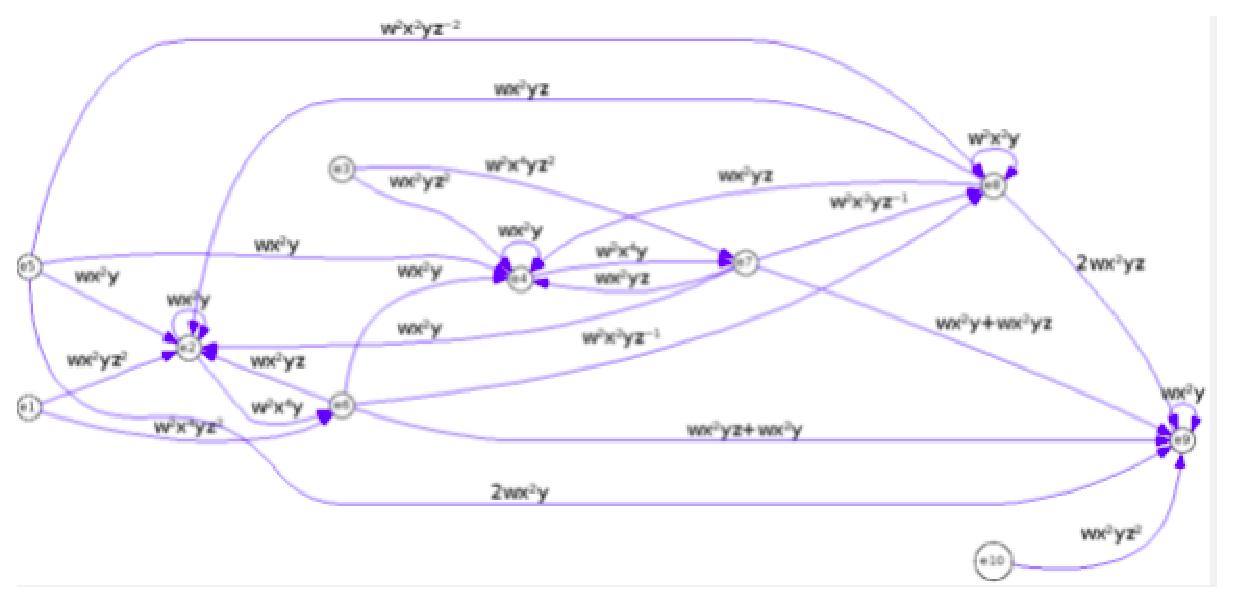
\includegraphics[width=15cm,height=10cm]{A2F2.eps}
%\begin{figure}[!htb]
\begin{minipage}[c]{.01\linewidth}
 \centering
 
 \end{minipage}
 \begin{minipage}[c]{.40\linewidth}
 \centering
 \begin{tikzpicture}[shorten >=1pt,node distance=3cm,initial text=,auto]
  \tikzstyle{every state}=[fill={rgb:black,1;white,10}]
  \node[state,initial]   (e_1)                       {$e_1$};
  \node[state,initial]           (e_5) [above of=e_1] {$e_5$};
   \node[state,initial]           (e_3) [above of=e_5]  {$e_3$};
  \node[state]           (e_4) [right of=e_5] {$e_4$};
  \node[state]           (e_2) [below right of= e_5]     {$e_2$};
  \node[state,accepting] (e_6) [ below right of=e_2]  {$e_6$};
  \node[state,accepting] (e_7) [right of= e_4]  {$e_7$};
  \node[state,accepting] (e_8) [above right of= e_7]  {$e_8$};
  \node[state,accepting] (e_9) [below right of=e_8]  {$e_9$};
  \node[state]           (e_{10}) [below of= e_9]     {$e_{10}$};

  \path[->]
  (e_1)   edge              node {$T_{1,2}$} (e_2)
        edge              node {$T_{1,6}$} (e_6)
  (e_2)  edge              node {$T_{2,6}$} (e_6)
   (e_3)     edge  [bend right] node {$T_{3,4}$} (e_4)
        edge  [bend left]     node {$T_{3,7}$} (e_7)
        
  (e_4) edge [loop above]  node {$T_{4,4}$} (   )
  (e_8) edge [loop right]  node {$T_{8,8}$} (   )
  (e_9) edge [loop right]  node {$T_{9,9}$} (   )
  (e_2) edge [loop above]  node {$T_{2,2}$} (   )
  (e_4)     edge [bend left]  node {$T_{4,7}$} (e_7)
   (e_5)     edge              node {$T_{5,2}$} (e_2)
             edge              node {$T_{5,4}$} (e_4)
             edge [bend left]             node {$T_{5,8}$} (e_8)
             edge [bend right]  node {$T_{5,9}$} (e_9)
    (e_6)    edge [bend left]  node {$T_{6,2}$} (e_2)
             edge [bend right] node {$T_{6,8}$} (e_8)
             edge [bend right]  node {$T_{6,4}$} (e_4)
             edge [bend right]  node {$T_{6,9}$} (e_9)
   (e_7)    edge [bend left]  node {$T_{7,2}$} (e_2)
            edge [bend left]  node {$T_{7,4}$} (e_4)
            edge [bend left]  node {$T_{7,8}$} (e_8)
            edge [bend left]  node {$T_{7,9}$} (e_9)
   (e_8)    edge [bend left]  node {$T_{8,2}$} (e_2)
            edge [bend right]  node {$T_{8,4}$} (e_4)
            edge [bend left]  node {$T_{8,9}$} (e_9)
   (e_{10}) edge [bend right]  node {$T_{10,9}$} (e_9);
\end{tikzpicture}
\end{minipage}
\caption{\label{Atfig12} Automate $\mathcal{A}_{2}$.}
\end{figure}
%\end{figure} 
\begin{spacing}{0.30}
\subsection*{Les transitions impossibles et les raisons pour lesquelles elles le sont}
\end{spacing}
\begin{spacing}{0.30}
\subsubsection*{Compte tenu de la proposition \ref{prop1} (perte de la connexité)}
\end{spacing}
$e_{1}\rightarrow e_{3}$, $e_{2}\rightarrow e_{3}$, $e_{3}\rightarrow e_{1}$, $e_{3}\rightarrow e_{2}$, $e_{1}\rightarrow e_{4}$, $e_{2}\rightarrow e_{4}$, $e_{4}\rightarrow e_{1}$ et $e_{4}\rightarrow e_{2}$.
\begin{spacing}{0.30}
\subsubsection*{Compte tenu de la proposition \ref{propdec191}}
\end{spacing}
$e_{1}\rightarrow e_{1}$, $e_{2}\rightarrow e_{1}$, $e_{5}\rightarrow e_{1}$, $e_{6}\rightarrow e_{1}$, $e_{7}\rightarrow e_{1}$, $e_{8}\rightarrow e_{1}$, $e_{3}\rightarrow e_{3}$, $e_{4}\rightarrow e_{3}$, $e_{5}\rightarrow e_{3}$, $e_{6}\rightarrow e_{3}$, $e_{7}\rightarrow e_{3}$, $e_{8}\rightarrow e_{3}$, $e_{1}\rightarrow e_{5}$, $e_{2}\rightarrow e_{5}$, $e_{3}\rightarrow e_{5}$, $e_{4}\rightarrow e_{5}$, $e_{5}\rightarrow e_{5}$, $e_{6}\rightarrow e_{5}$, $e_{7}\rightarrow e_{5}$, $e_{8}\rightarrow e_{5}$, $e_{3}\rightarrow e_{6}$, $e_{4}\rightarrow e_{6}$, $e_{5}\rightarrow e_{6}$, $e_{6}\rightarrow e_{6}$, $e_{7}\rightarrow e_{6}$, $e_{8}\rightarrow e_{6}$, $e_{1}\rightarrow e_{7}$, $e_{2}\rightarrow e_{7}$, $e_{5}\rightarrow e_{7}$, $e_{6}\rightarrow e_{7}$, $e_{7}\rightarrow e_{7}$, $e_{8}\rightarrow e_{7}$, $e_{1}\rightarrow e_{8}$, $e_{2}\rightarrow e_{8}$, $e_{3}\rightarrow e_{8}$, $e_{4}\rightarrow e_{8}$, $e_{9}\rightarrow e_{10}$ et $e_{2}\rightarrow e_{10}$.
\begin{spacing}{0.30}
\subsubsection*{Compte tenu de la proposition \ref{prop2606221}}
\end{spacing}
$e_{1}\rightarrow e_{9}$, $e_{2}\rightarrow e_{9}$, $e_{3}\rightarrow e_{9}$ et $e_{4}\rightarrow e_{9}$.
\begin{spacing}{0.30}
\subsubsection*{Compte tenu des propositions \ref{prop2606221} et \ref{propdec191}}
\end{spacing}
$e_{1}\rightarrow e_{10}$, $e_{2}\rightarrow e_{10}$, $e_{3}\rightarrow e_{10}$ et $e_{4}\rightarrow e_{10}$.
\begin{spacing}{0.30}
\subsubsection*{Compte tenu des propositions \ref{prop3} et \ref{propdec191}}
\end{spacing}
$e_{9}\rightarrow e_{1}$, $e_{9}\rightarrow e_{2}$, $e_{9}\rightarrow e_{3}$, $e_{9}\rightarrow e_{4}$,   $e_{9}\rightarrow e_{5}$, $e_{9}\rightarrow e_{6}$, $e_{9}\rightarrow e_{7}$, $e_{9}\rightarrow e_{8}$, $e_{10}\rightarrow e_{1}$, $e_{10}\rightarrow e_{2}$, $e_{10}\rightarrow e_{3}$, $e_{10}\rightarrow e_{4}$, $e_{10}\rightarrow e_{5}$, $e_{10}\rightarrow e_{6}$, $e_{10}\rightarrow e_{7}$ et $e_{10}\rightarrow e_{8}$.
\begin{spacing}{0.30}
\section{Automate $\mathcal{A}_{3}$}
\end{spacing}
$\mathcal{A}_{3}$ a $12$ classes d'états qui sont présentées ci-dessous.
\begin{eqnarray*}
& & cl_{1} = (100,\{\{0\}\}), \quad cl_{2} = (010,\{\{0\}\}), \quad cl_{3}=(001,\{\{0\}\}),\\
& &cl_{4}=(110,\{\{0\}\}),\quad cl_{5}=(101,\{\{0,1\}\}),\quad cl_{6} = (101,\{\{0\},\{1\}\}), \\
& &cl_{7} = (011,\{\{0\}\}),\quad cl_{8}=(111,\{\{0\}\}),\quad cl_{9}=(10,\{\{0\}\}),\\
& & cl_{10}=(01,\{\{0\}\}),\quad cl_{11} =(11,\{\{0\}\})\textit{ et }\quad cl_{12}=(1,\{\{0\}\}).
\end{eqnarray*} 
On a donc les états suivants
\small
\begin{longtable}{|c|c|c|} 
\hline
$e_{1}=(100,000,\{\{0\}\})$&
$e_{2}=(100,100,\{\{0\}\})$&
$e_{3}=(010,000,\{\{0\}\})$\\
$e_{4}=(010,010)\{\{0\}\})$&
$e_{5}=(001,000,\{\{0\}\}$&
$e_{6}=(001,001,\{\{0\}\})$\\
$e_{7}=(110,110,\{\{0\}\})$&
$e_{8}=(110,210,\{\{0\}\})$&
$e_{9}=(110,120,\{\{0\}\})$\\
$e_{10}=(110,220,\{\{0\})$&
$e_{11}=(101,000,\{\{0\},\{1\}\})$& 
$e_{12}=(101,101,\{\{0\},\{1\}\})$ \\
$e_{13}=(101,100,\{\{0\},\{1\}\})$& 
$e_{14}=(101,001,\{\{0\},\{1\})$&
$e_{15}=(101,101,\{\{0,1\}\})$ \\
$e_{16}=(011,011,\{\{0\}\})$&
$e_{17}=(011,021,\{\{0\}\})$&
$e_{18}=(011,012,\{\{0\}\})$\\
$e_{19}=(011,022,\{\{0\}\})$&
$e_{20}=(111,121,\{\{0\}\})$&
$e_{21}=(111,221,\{\{0\}\})$\\
$e_{22}=(111,122,\{\{0\}\})$&
$e_{23}=(111,222,\{\{0\}\})$&
$e_{24}=(111,131,\{\{0\}\})$\\
$e_{25}=(111,231,\{\{0\}\})$&
$e_{26}=(111,132,\{\{0\}\})$&
$e_{27}=(111,232,\{\{0\}\})$\\
$e_{28}=(10,00,\{\{0\}\})$&
$e_{29}=(10,10,\{\{0\}\})$&
$e_{30}=(01,00,\{\{0\}\})$\\
$e_{31}=(01,01,\{\{0\}\})$&
$e_{32}=(11,11,\{\{0\}\})$&
$e_{33}=(11,21,\{\{0\}\})$\\
$e_{34}=(11,12,\{\{0\}\})$&
$e_{35}=(11,22,\{\{0\}\})$&
$e_{36}=(1,0,\{\{0\}\})$ \\
$e_{37}=(1,1,\{\{0\}\})$ & &\\
\hline
\caption{\label{tab6} Les états de $\mathcal{A}_{3}$.}
\end{longtable}
\normalsize
 
 Les transitions possibles sont les suivantes:
 \small
\begin{longtable}{|c|c|} 
\hline
$T_{1,2}= yz^2wx^2$\quad\quad \quad &

$T_{1,8}= yz^2w^2x^4$\\

$T_{1,13}= yz^2w^2x^6$ &

$T_{1,21}= yz^2w^3x^6$\\

$T_{2,2}= ywx^2$&

$T_{2,8}= yw^2x^4$\\

$T_{2,13}= yw^2x^6$&

$T_{2,21}= yw^3x^6$\\

$T_{3,4}= yz^2wx^2$&

$T_{3,9}= yz^2w^2x^4$\\

$T_{3,17}= yz^2w^2x^4$&

$T_{3,24}= yz^3w^3x^6$\\

$T_{4,4}= ywx^2$&

$T_{4,9}= yw^2x^4$\\

$T_{4,17}= yw^2x^4$&

$T_{4,24}= yzw^3x^6$\\

$T_{5,6}= yz^2wx^2$&

$T_{5,14}= yz^2w^2x^6$\\

$T_{5,18}= yz^2w^2x^4$&

$T_{5,22}= yz^2w^3x^6$\\

$T_{6,6}= ywx^2$&

$T_{6,14}= yw^2x^6$\\

$T_{6,18}= yw^2x^4$&

$T_{6,22}= yw^3x^6$\\

$T_{7,2}= ywx^2$&

$T_{7,4}= ywx^2$\\

$T_{7,10}= yz^{-2}w^2x^2$&

$T_{7,13}= yw^2x^6$\\

$T_{7,17}= yw^2x^4$&

$T_{7,25}= yz^{-1}w^3x^4$\\

$T_{7,29}= ywx^2$&

$T_{7,33}= yw^2x^4$\\

$T_{8,2}= yzwx^2$&

$T_{8,4}= ywx^2$\\

$T_{8,10}= yz^{-1}w^2x^2$&

$T_{8,13}= yzw^2x^6$\\

$T_{8,17}= yw^2x^4$&

$T_{8,25}= yw^3x^4$\\

$T_{8,29}= ywx^2$&

$T_{8,33}= yw^2x^4$\\

$T_{9,2}= ywx^2$&

$T_{9,4}= yzwx^2$\\

$T_{9,10}= yz^{-1}w^2x^2$&

$T_{9,13}= yw^2x^6$\\

$T_{9,17}= yzw^2x^4$&

$T_{9,25}= yw^3x^4$\\

$T_{9,29}= yzwx^2$&

$T_{9,33}= yzw^2x^4$\\

$T_{10,2}= yzwx^2$&

$T_{10,4}= yzwx^2$\\

$T_{10,10}= yw^2x^2$ &

$T_{10,13}= yzw^2x^6$\\

$T_{10,17}= yzw^2x^4$&

$T_{10,25}= yzw^3x^4$\\

$T_{10,29}= yzwx^2$&

$T_{10,33}= yzw^2x^4$\\

$T_{11,12}= yz^4w^2x^4$&

$T_{11,23}= yz^2w^3x^4$\\

$T_{12,12}= yw^2x^4$&

$T_{12,23}= yz^{-2}w^3x^4$\\
 
$T_{13,12}= yz^2w^2x^4$& 

$T_{13,23}= yzw^3x^4$\\

$T_{14,12}= yz^2w^2x^4$ &

$T_{14,23}= yw^3x^4$\\

$T_{15,2}= ywx^2$&

$T_{15,6}= ywx^2$\\

$T_{15,8}= yw^2x^4$&

$T_{15,15}= yw^2x^4$\\

$T_{15,18}= yw^2x^4$ &

$T_{15,23}= yz^{-2}w^3x^4$\\

$T_{15,29}= ywx^2$&

$T_{15,31}= ywx^2$\\

$T_{15,33}= yw^2x^4$&

$T_{15,34}= yw^2x^4$\\

$T_{15,37}= 2ywx^2$&

$T_{16,4}= ywx^2$\\

$T_{16,6}= ywx^2$ &

$T_{16,9}= yw^2x^4$\\

$T_{16,14}= yw^2x^6$&

$T_{16,19}= yz^{-2}w^2x^2$\\

$T_{16,26}= yz^{-1}w^3x^4$\quad\quad \quad &

$T_{16,31}= ywx^2$\\

$T_{16,34}= yw^2x^4$&

$T_{17,4}= yzwx^2$\\

$T_{17,6}= ywx^2$&

$T_{17,9}= yzw^2x^4$\\

$T_{17,14}= yw^2x^6$&

$T_{17,19}= yz^{-1}w^2x^2$\\

$T_{17,26}= yw^3x^4$&

$T_{17,31}= yzwx^2$ \\

$T_{17,34}= yzw^2x^4$&

$T_{18,4}= ywx^2$\\

$T_{18,6}= yzwx^2$&

$T_{18,9}= yw^2x^4$\\

$T_{18,14}= yzw^2x^6$&

$T_{18,19}= yz^{-1}w^2x^2$\\

$T_{18,26}= yw^3x^4$&

$T_{18,31}= ywx^2$\\

$T_{18,34}= yw^2x^4$&

$T_{19,4}= yzwx^2$\\

$T_{19,6}= yzwx^2$&

$T_{19,9}= yzw^2x^4$\\

$T_{19,14}= yzw^2x^6$&

$T_{19,19}= yw^2x^2$\\

$T_{19,26}= yzw^3x^4$&

$T_{19,31}= yzwx^2$\\

$T_{19,34}= yzw^2x^4$&

$T_{20,2}= ywx^2$\\

$T_{20,4}= yzwx^2$&

$T_{20,6}= ywx^2$\\

$T_{20,10}= yz^{-1}w^2x^2$&

$T_{20,15}= yw^2x^4$\\

$T_{20,19}= yz^{-1}w^2x^2$&

$T_{20,27}= yz^{-2}w^3x^2$\\

$T_{20,29}= yzwx^2+ywx^2$&

$T_{20,31}= yzwx^2+ywx^2$\\

$T_{20,35}= 2yz^{-1}w^2x^2$ &

$T_{20,37}= 2yw^2x^2+yz^{-1}w^2x^2$\\

$T_{21,2}= yzwx^2$&

$T_{21,4}= yzwx^2$ \\
$T_{21,6}= ywx^2$&

$T_{21,10}= yw^2x^2$ \\

$T_{21,15}= yzw^2x^4$ &

$T_{21,19}= yz^{-1}w^2x^2$\\

$T_{21,27}= yz^{-1}w^3x^2$ &

$T_{21,31}= yzwx^2+ywx^2$\\ 
$T_{21,29}= 2yzwx^2$ &

$T_{21,35}= yw^2x^2+yz^{-1}w^2x^2$\\

$T_{21,37}= 2yzwx^2+ywx^2$ &

$T_{22,2}= ywx^2$\\

$T_{22,4}= yzwx^2$&

$T_{22,6}= yzwx^2$ \\

$T_{22,10}= yz^{-1}w^2x^2$&

$T_{22,15}= yzw^2x^4$\\

$T_{22,19}= yw^2x^2$&

$T_{22,27}= yz^{-1}w^3x^2$\\

$T_{22,29}= yzwx^2+ywx^2$& 

$T_{22,31}= 2yzwx^2$ \\

$T_{22,35}= yw^2x^2+yz^{-1}w^2x^2$ &

$T_{22,37}= 2yzwx^2+ywx^2$\\

$T_{23,2}= yzwx^2$ &

$T_{23,4}= yzwx^2$\\

$T_{23,6}= yzwx^2$&

$T_{23,10}= yw^2x^2$ \\

$T_{23,15}= yz^2w^2x^4$&

$T_{23,19}= yw^2x^2$\\

$T_{23,27}= yw^3x^2$&

$T_{23,29}= 2yzwx^2$\\

$T_{23,31}= 2yzwx^2$&

$T_{23,35}= 2yw^2x^2$\\

$T_{23,37}= 3yzwx^2$&

$T_{24,2}= ywx^2$\\

$T_{24,4}= yzwx^2$&

$T_{24,6}= ywx^2$\\

$T_{24,10}= yz^{-1}w^2x^2$&

$T_{24,15}= yw^2x^4$ \\

$T_{24,19}= yz^{-1}w^2x^2$&

$T_{24,27}= yz^{-2}w^3x^2$\\ 

$T_{24,29}= yzwx^2+ywx^2$ &

$T_{24,31}= yzwx^2+ywx^2$\\ 

$T_{24,35}= 2yz^{-1}w^2x^2$&

$T_{24,37}= yzwx^2+2ywx^2$ \\

$T_{25,2}= yzwx^2$&

$T_{25,4}= yzwx^2$\\

$T_{25,6}= ywx^2$&

$T_{25,10}= yw^2x^2$\\

$T_{25,15}= yzw^2x^4$&

$T_{25,19}= yz^{-1}w^2x^2$\\

$T_{25,27}= yz^{-1}w^3x^2$&

$T_{25,29}= 2yzwx^2$\\

$T_{25,31}= yzwx^2+ywx^2$ & 

$T_{25,35}= yw^2x^2+yz^{-1}w^2x^2$\\

$T_{25,37}= 2yzwx^2+ywx^2$& 

$T_{26,2}= ywx^2$ \\

$T_{26,4}= yzwx^2$&

$T_{26,6}= yzwx^2$ \\

$T_{26,10}= yz^{-1}w^2x^2$ &

$T_{26,15}= yzw^2x^4$\\ 

$T_{26,19}= yw^2x^2$ &

$T_{26,27}= yz^{-1}w^3x^2$ \\

$T_{26,29}= yzwx^2+ywx^2$&

$T_{26,31}= 2yzwx^2$\\

$T_{26,35}= yw^2x^2+yz^{-1}w^2x^2$&

$T_{26,37}= 2yzwx^2+ywx^2$\\

$T_{27,2}= yzwx^2$&

$T_{27,4}= yzwx^2$\\

$T_{27,6}= yzwx^2$&

$T_{27,10}= yw^2x^2$\\

$T_{27,15}= yz^2w^2x^4$&

$T_{27,19}= yw^2x^2$\\

$T_{27,27}= yw^3x^2$&

$T_{27,29}= 2yzwx^2$\\

$T_{27,31}= 2yzwx^2$&

$T_{27,35}= 2yw^2x^2$\\

$T_{27,37}= 3yzwx^2$&

$T_{28,29}= yz^2wx^2$\\

$T_{28,33}= yz^2w^2x^4$&

$T_{29,29}= ywx^2$\\

$T_{29,33}= yw^2x^4$&

$T_{30,31}= yz^2wx^2$\\

$T_{30,34}= yz^2w^2x^4$&

$T_{31,31}= ywx^2$\\

$T_{31,34}= yw^2x^4$&

$T_{32,29}= ywx^2$\\

$T_{32,31}= ywx^2$&

$T_{32,35}= yz^{-2}w^2x^2$\\

$T_{32,37}= 2ywx^2$&

$T_{33,29}= yzwx^2$\\

$T_{33,31}= ywx^2$&

$T_{33,35}= yz^{-1}w^2x^2$\\

$T_{33,37}= yzwx^2+ywx^2$&

$T_{34,29}= ywx^2$\\

$T_{34,31}= yzwx^2$&

$T_{34,35}= yz^{-1}w^2x^2$\\

$T_{34,37}= yzwx^2+ywx^2$&

$T_{35,29}= yzwx^2$\\

$T_{35,31}= yzwx^2$&

$T_{35,35}= yw^2x^2$\\

$T_{35,37}= 2yzwx^2$&

$T_{36,37}= yz^2wx^2$\\

$T_{37,37}= ywx^2$& \\
\hline
\caption{\label{tab3} Les transitions possibles de $\mathcal{A}_{3}$.}
\end{longtable} 
\normalsize
Les états initiaux de $\mathcal{A}_{3}$ sont $e_{1}$, $e_{3}$, $e_{5}$, $e_{7}$, $e_{11}$, $e_{16}$,  $e_{20}$.  Ses états finaux  sont $e_{15}$, $e_{21}$, $e_{22}$, $e_{23}$, $e_{24}$, $e_{25}$,  $e_{26}$, $e_{27}$, $e_{33}$, $e_{34}$, $e_{35}$, $e_{37}$.       
\section{Validation des valeurs dans les matrices de transfert $\mathcal{M}_{2}$ et $\mathcal{M}_{3}$}
Dans cette section nous vérifions si les entrées des matrices $\mathcal{M}_{2}$ et $\mathcal{M}_{3}$ sont fiables, c'est-à-dire si la somme des coefficients des entrées $a_{i,j}$  de la  matrice $\mathcal{M}_{2}^{n}$ ( ou  $\mathcal{M}_{3}^{n}$), où $n$ est un entier naturel supérieur ou égal à $0$, correspond à la $(n+1)^{ieme}$ valeur de  la suite du nombre de polyominos inscrits dans le rectangle de type $2$ (ou de type $3$) sur  \emph{The On-Line Encyclopedia of Integer Sequences} \citep{Oeis,Oeis2}. Pour cela, nous calculons la matrice $M_{2}^{n}$ (respectivement $M_{3}^{n}$) et comparons la somme $S_{n}$ des coefficients des polynômes correspondants aux entrées $a_{i,j}$ de cette dernière. On note que $a_{i,j}$ est une transition de  l'état initial $e_{i}$ à l'état final  $e_{j}$.
\subsection{Validation des valeurs de la matrice $\mathcal{M}_{2}$}
\begin{itemize}
\item[(i)] Cas $n=0$

Dans ce cas particulier, il s'agit de trouver l'unique polyomino inscrit dans le rectangle de base $B=2$ et de hauteur $1$ (voir figure \ref{uni2}). La valeur de $S_{0}$ vaut particulièrement $1$ dans ce cas.
 \begin{figure}[!htb]
 \begin{minipage}[c]{.26\linewidth}
  \centering
  \end{minipage}
  \hfill
\begin{minipage}[c]{.56\linewidth}
  \centering
\begin{logicpuzzle}[rows=1,columns=2,color=cyan!100, width=750px,scale=0.5]
\fillcell{1}{1}
\fillcell{2}{1}
\framepuzzle[black!50]
\end{logicpuzzle}
\end{minipage}
\caption{\label{uni2} Polyomino inscrit dans le rectangle $2\times 1$.}
\end{figure}
\item[(ii)] Cas $n=1$

Il suffit, dans ce cas, de faire la somme $S_{1}$ des coefficients des polynômes de Laurent des entrées $m_{i,j}$ de la matrice $\mathcal{M}_{2}$  correspondantes aux transitions des états initiaux aux états finaux. Dans le tableau ci-dessous, nous listons les entrées  non nulles correspondantes aux transitions d'états initiaux aux états finaux.\\

\begin{tabular}{|c|c|c|c|}
 \hline
  Transition& $m_{i,j}$ & Somme  coefficients\\
 \hline
 $e_{1}\rightarrow e_{6}$ & $w^{2}x^{4}yz^{2}$ & $1$ \\
 \hline
 $e_{3}\rightarrow e_{7}$ & $w^{2}x^{4}yz^{2}$ & $1$ \\
 \hline
 $e_{5}\rightarrow e_{8}$ & $w^{2}x^{2}yz^{-2}$ & $1$ \\
 \hline
 $e_{5}\rightarrow e_{9}$ & $2wx^{2}y$ & $2$ \\
 \hline
\end{tabular}
\mbox{ }\\
$S_{1}=1+1+1+2=5$. Ce qui signifie qu'on a au total $5$ polyominos inscrits dans le carré $2\times 2$.
\item[(iii)] Cas $n=2$

 Nous faisons la  somme $S_{2}$ des coefficients des polynômes de Laurent des entrées $m_{i,j}$ de la matrice $\mathcal{M}_{2}^{2}$  correspondantes aux transitions des états initiaux aux états finaux.
 
 \begin{tabular}{|c|c|c|c|}
 \hline
  Transition & $m_{i,j}$&Somme  coefficients\\
 \hline
  $e_{1}\rightarrow e_{6}$ & $w^3x^6y^2z^{2}$ &$1$ \\ 
 \hline
 $e_{1}\rightarrow e_{8}$ & $w^4x^6y^2z$  & $1$ \\
 \hline
 $e_{1}\rightarrow e_{9}$ & $w^3x^6y^2z^{3}+w^3x^6y^2z^{2}$ & $2$ \\
 \hline
 $e_{3}\rightarrow e_{7}$ & $w^3x^6y^2z^{2}$ & $1$ \\
 \hline
 $e_{3}\rightarrow e_{8}$ & $ w^4x^6y^2z$ & $1$ \\
 \hline
 $e_{3}\rightarrow e_{9}$ & $w^3x^6y^2z^{3}+w^3x^6y^2z^{2} $\ & $2$ \\
 \hline
  $e_{5}\rightarrow e_{6}$&$ w^3x^6y^2 $& $1$\\
 \hline
  $e_{5}\rightarrow e_{7}$&$ w^3x^6y^2, $& $1$\\
 \hline
  $e_{5}\rightarrow e_{8}$&$ w^4x^4y^2z^{-2}  $& $1$\\
 \hline
  $e_{5}\rightarrow e_{9}$&$2w^3x^4y^2z^{-1}+2w^2x^4y^2$& $4$\\
 \hline
\end{tabular}
\mbox{ }\\\\
$S_{2}=1+1+2+1+1+2+1+1+1+4=15$.

\item[(iv)] Cas $n=3$\\
 Nous listons les entrées $m_{i,j}$ non nulles, $i\in\{1,3,5\}$ et $j\in\{6,7,8,9\}$. 
 On a 
 
$m_{1,6}=w^4x^8y^3z^2+w^5x^{10}y^3z^3$,  $m_{1,7}=w^5x^{10}y^3z^2 $,  $m_{1,8}=w^5x^8y^3z+w^6x^8y^3z$,  $m_{1,9}=2w^5x^8y^3z^2+2w^4x^8y^3z^3+2w^4x^8y^3z^2$,
$m_{3,6}=w^5x^{10}y^3z^2$, $m_{3,7}=w^4x^8y^3z^2+w^5x^{10}y^3z^3 $,  $m_{3,8}=w^5x^8y^3z+w^6x^8y^3z$,  $m_{3,9}=2w^5x^8y^3z^2+2w^4x^8y^3z^3+2w^4x^8y^3z^2$, 
$m_{5,6}=w^4x^8y^3+w^5x^8y^3z^{-1}$, $m_{5,7}=w^4x^8y^3+w^5x^8y^3z^{-1}$,$m_{5,8}=2w^5x^8y^3z^{-1}+w^6x^6y^3z^{-2}$, $m_{5,9}=2w^3x^6y^3+2w^4x^6y^3z^{-1}+2w^4x^8y^3+2w^4x^8y^3z+2w^5x^6y^3z^{-1}$.

$S_{3}=2+1+2+6+1+2+2+6+2+2+3+10=39$.

\item[(v)] Cas $n=4$\\

$m_{1,6}=w^7x^{12}y^4z^{2}+2w^6x^{12}y^4z^{3}+w^5x^{10}y^4z^{2}$, $m_{1,7}=w^7x^{12}y^4z^{2}+2z^2w^6x^{12}y^4$, $m_{1,8}=w^7x^{12}y^4z^2+w^7x^{10}y^4z+w^8x^{10}y^4z+w^7x^{12}y^4z+w^6x^{10}y^4z$, $m_{1,9}=2z^2w^7x^{10}y^4+2z^3w^6x^{12}y^4+w^6x^{12}y^4z^{2}+4z^2w^6x^{10}y^4+3z^2w^5x^{10}y^4+w^6x^{12}y^4z^{3}+3w^5x^{10}y^4z^{3}$,  $m_{3,6}=w^7x^{12}y^4z^{2}+2w^6x^{12}y^4z^{2}$, $m_{3,7}=w^7x^{12}y^4z^{2}+2z^3w^6x^{12}y^4+z^2w^5x^{10}y^4$, $m_{3,8}=w^7x^{12}y^4z^{2}+w^7x^{10}y^4z+w^8x^{10}y^4z+w^7x^{12}y^4z+w^6x^{10}y^4z$, $m_{3,9}=2w^7x^{10}y^4z^{2}+2w^6x^{12}y^4z^{3}+w^6x^{12}y^4z^{2}+4z^2w^6x^{10}y^4+3w^5x^{10}y^4z^{2}+w^6x^{12}y^4z^{4}+3w^5x^{10}y^4z^{3}$, $m_{5,6}=w^6x^{12}y^4+w^5x^{10}y^4+w^7x^{10}y^4z^{-1}+w^6x^{12}y^4z+w^6x^{10}y^4z^{-1}$, $m_{5,7}=w^6x^{12}y^4+w^5x^{10}y^4+w^7x^{10}y^4z^{-1}+w^6x^{12}y^4z+w^6x^{10}y^4z^{-1}$,  $m_{5,8}=
2w^7x^{10}y^4z^{-2}+2w^7x^{10}y^4z^{-1}+w^8x^8y^4z^{-2}+2w^6x^{10}y^4z^{-1}$, $m_{5,9}= 2w^6x^8y^4z^{-1}+4w^5x^{10}y^4z+2w^4x^8y^4+6w^6x^{10}y^4+2w^7x^8y^4z^{-1}+4w^5x^{10}y^4z^{-1}+2w^5x^8y^4z^{-1}+2w^6x^{10}y^4z^{-1}$.
\mbox{ }\\\\
$S_{4}=4+3+5+16+3+4+5+16+5+5+7+24=97$.
\item[(vi)] Cas $n=5$\\

Pour ce cas, étant donné que les expressions des entrées $m_{i,j}$ de la matrice $\mathcal{M}_{2}^{5}$ sont de très grandes tailles, pour chacune d'elles, nous donnons la somme des coefficients  de ses monômes.\\\\
 \tiny
\begin{tabular}{|c|c|c|c|c|c|c|c|c|c|c|c|c|}
 \hline
Entrées & $m_{1,6}$& $m_{1,7}$&$m_{1,8}$ & $m_{1,9}$& $m_{3,6}$ &$m_{3,7}$ & $m_{3,8}$&$m_{3,9}$ & $m_{5,6}$& $m_{5,7}$ &$m_{5,8}$ &$m_{5,9}$ \\
 \hline
 coef  &$9$ &$8$&$12$ &$40$  &$8$ &$9$ &$12$  &$40$&$12$ &$12$  &$17$&$58$ \\
 \hline
 \end{tabular}
 \normalsize
\mbox{ }\\\\
$S_{5}=9+8+12+40+8+9+12+40+12+12+17+58=237$.
\end{itemize}
Dans le tableau \ref{v2} nous listons, pour chaque valeur $n$, $1\leq n\leq 15$, le nombre  polyominos inscrits dans le rectangle de base $2$ et de hauteur $H=n+1$. Pour chaque valeur $n$, $s_{1}$, $s_{2}$ et $s_{5}$ désigne respectivement les nombres de polyominos obtenus à partir des états initiaux $e_{1}$, $e_{3}$ et $e_{5}$ tandis-que $S_{n}$ est le nombre total de polyominos inscrits dans le rectangle $2\times (n+1)$.
\begin{small}
\begin{longtable}{|c|c|c|c|c|c|c|c|c|c|c|} 
\hline
$n$&$s_{1}$&$s_{3}$&$s_{5}$&$S_{n}$\\
\hline
$1$& $ 1 $&  $1 $& $ 2$&$ 5$\\
\hline
$2$& $ 4$& $ 4$& $ 7$&$15 $\\
\hline
$3$& $11 $& $11 $& $17 $&$39 $\\
\hline39
$4$& $ 28$& $28 $& $ 41$&$ 97$\\
\hline
$5$& $69 $& $69 $& $99 $&$237 $\\
\hline
$6$& $168$& $168$& $279$&$575$\\
\hline
$7$&$407$ &$407$ &$577$ &$1391$\\
\hline
$8$&$984$ & $984$&$1393$ &$ 3361
$\\
\hline
$9$& $2377$& $2377$&$3363$ &$8117$\\
\hline
$10$&$5740$ &$5740$ & $8119$&$19599$\\
\hline
$11$& $13859$&$13859$ & $19601$&$47319$\\
\hline
$12$&$33460$ & $33460$& $47321$&$114241$\\
\hline
$13$&$80781$ & $80781$& $114243$&$275805
$\\
\hline
$14$&$195024$ & $195024$&$275807$ &$665855$\\
\hline
$15$& $470831$&$470831$& $665857$&$1607519$\\
\hline
\caption{\label{v2} Nombres de polyominos inscrits dans quelques rectangles de type $2$.}
\end{longtable}
\end{small}
À travers les quinze cas présentés  ci-dessus, nous avons obtenu les quinze premières valeurs de la suite numéro $A034182 $ des nombres de polyominos inscrits dans un rectangle de base $2$ du site \emph{OEIS}. Sur la base de ces résultats, nous conjecturons que pour toute valeur de $n\geq 5$, la $(n+1)^{ieme}$ valeur de la suite des nombres de polyominos inscrits dans un rectangle de largeur $2$ est la même que celle de \emph{OEIS}.
\begin{spacing}{0.30}
\subsection{Validation des valeurs de la matrice $\mathcal{M}_{3}$}
\end{spacing}
Tout comme la section précédente, nous calculons, en utilisant les puissances de la matrice $\mathcal{M}_{3}$, les sept premières valeurs de la suite des nombres de polyominos inscrits dans un rectangle du type $3$ tout en les comparant à celles de l'\emph{OEIS}. On rappelle que  l'automate $\mathcal{A}_{3 }$ a pour   états  initiaux les états $e_{1}, e_{3}, e_{5}, e_{7}, e_{11}, e_{16}, e_{20}$ et pour états finaux les états $e_{15},  e_{21}, e_{22}, e_{23}, e_{24}, e_{25}$, $ e_{26}, e_{27}, e_{33}, e_{34},  e_{35},  e_{37}. $

Pour chaque état initial $e_{i}$ de $\mathcal{A}_{3}$, nous calculons la somme $s_{i}$ des coefficients de toutes les entrées $m_{i,j}$ de la matrice $\mathcal{M}_{3}^{n}$, correspondantes aux suites de transitions de $e_{i}$ à $e_{j}$, $j\in \{15, 21, 22, 23, 24, 25, 26, 27, 33, 34, 35, 37\}$. On désigne par  $S_{n}$ la somme des $s_{i}$, $i$ parcourant l'ensemble des indices des états initiaux de $\mathcal{A}_{3}$.
\begin{itemize}
\item[(i)] Cas $n=0$
Dans ce cas particulier, il s'agit de trouver l'unique polyomino inscrit dans le rectangle de type $B=3$ et de hauteur $1$ (voir figure \ref{uni3}). La valeur de $S_{0}$ vaut particulièrement $1$ dans ce cas.
 \begin{figure}[!htb]
 \begin{minipage}[c]{.26\linewidth}
  \centering
  \end{minipage}
  \hfill
\begin{minipage}[c]{.56\linewidth}
  \centering
\begin{logicpuzzle}[rows=1,columns=3,color=cyan!100, width=750px,scale=0.5]
\fillcell{1}{1}
\fillcell{2}{1}
\fillcell{3}{1}
\framepuzzle[black!50]
\end{logicpuzzle}
\end{minipage}
\caption{\label{uni3} Polyomino inscrit dans le rectangle $3\times 1$.}
\end{figure}
\item[(ii)] Cas $n=1$ (matrice $\mathcal{M}_{3}$)\\

\begin{tabular}{|c|c|c|c|c|c|c|c|c|c|c|c|c|}
 \hline
 $i$ & $1$ & $3$ & $5$ & $7$ & $11$ & $16$ & $20$&$S_{1}$\\
 \hline
 $s_{i}$ & $1$ & $1$ & $1$ & $2$ & $1$&$1$&$8$&$15$\\
 \hline
 \end{tabular}
 \mbox{ }\\
\item[(iii)] Cas $n=2$ (matrice $\mathcal{M}_{3}^{2}$)\\
\begin{tabular}{|c|c|c|c|c|c|c|c|c|c|c|c|c|}
 \hline
 $i$ & $1$ & $3$ & $5$ & $7$ & $11$ & $16$ & $20$&$S_{2}$\\
 \hline
 $s_{i}$ & $11$ & $12$ & $12$ & $18$ & $8$&$17$&$33$&$111$\\
 \hline
 \end{tabular}
 \mbox{ }\\
\item[(iv)] Cas $n=3$ (matrice $\mathcal{M}_{3}^{3}$)\\
\mbox{}\\
\begin{tabular}{|c|c|c|c|c|c|c|c|c|c|c|c|c|}
 \hline
 $i$ & $1$ & $3$ & $5$ & $7$ & $11$ & $16$ & $20$&$S_{3}$\\
 \hline
 $s_{i}$ & $70$ & $77$ & $74$ & $110$ & $41$&$111$&$166$&$749$\\
 \hline
 \end{tabular}
 \mbox{ }\\
\item[(v)] Cas $n=4$ (matrice $\mathcal{M}_{3}^{4}$)\\
\mbox{}\\
\begin{tabular}{|c|c|c|c|c|c|c|c|c|c|c|c|c|}
 \hline
 $i$ & $1$ & $3$ & $5$ & $7$ & $11$ & $16$ & $20$&$S_{4}$\\
 \hline
 $s_{i}$ & $387$ & $468$ & $387$ & $607$ & $206$&$607$&$833$&$3495$\\
 \hline
 \end{tabular}
 \mbox{ }\\
\item[(vi)] Cas $n=5$ (matrice $\mathcal{M}_{3}^{5}$)\\
\mbox{}\\
\begin{tabular}{|c|c|c|c|c|c|c|c|c|c|c|c|c|}
 \hline
 $i$ & $1$ & $3$ & $5$ & $7$ & $11$ & $16$ & $20$&$S_{5}$\\
 \hline
 $s_{i}$ & $2033$ & $2515$ & $2033$ & $3177$ & $1039$&$3177$&$4215$&$18189$\\
 \hline
 \end{tabular}
 \mbox{ }\\
\item[(vii)] Cas $n=6$ (matrice $\mathcal{M}_{3}^{6}$)\\
 \mbox{ }\\
 \begin{tabular}{|c|c|c|c|c|c|c|c|c|c|c|c|c|}
 \hline
 $i$ & $1$ & $3$ & $5$ & $7$ & $11$ & $16$ & $20$&$S_{6}$\\
 \hline
 $s_{i}$ & $10464$ & $13084$ & $10464$ & $16324$ & $5254$&$16324$&$21317$&$93231$\\
 \hline
 \end{tabular}
\end{itemize}
\mbox{}\\\mbox{}\\
Dans le tableau \ref{v3} nous listons, pour chaque valeur $n$, $1\leq n\leq 11$, le nombre  polyominos inscrits dans le rectangle de base $3$ et de hauteur $H=n+1$.
\begin{tiny}
\begin{longtable}{|c|c|c|c|c|c|c|c|c|c|c|} 
\hline
n&$s_{1}$&$s_{3}$&$s_{5}$&$s_{7}$&$s_{11}$&$s_{16}$&$s_{20}$&$S_{n}$\\
\hline
$1$& 1
 & 1
& 1 & 2
& 1
& 1
& 8& 15\\

\hline
$2$& 11
 & 12
& 12 & 18
& 8 
& 17
& 33 & 111\\

\hline
$3$& 70
 & 81
& 70 & 111
& 41
& 111
& 165 & 649\\

\hline
$4$& 387
 & 468
& 387 & 607
& 206
& 607
& 833& 3495\\

\hline
$5$& 2033
 & 2515
& 2033 & 3177
& 1039
& 3177
&4215 &18189\\
\hline
$6$& 10464
 & 13084
& 10464& 16324
& 5254
&16324 &
21317 &93231  \\
\hline
$7$&53359
 & 67049
& 53359& 83174
& 26571
&83174
 &  10779&474479\\
\hline
$8$&270897
 &341190
 &270897
 &422104
 &134364
 & 422104&545065 &2406621
\\
\hline
$9$&  1372430
&1730463
 &1372430
 & 2138101
& 679429
& 2138101
&2756183
 &12187137
\\
\hline
$10$&6946143
 &8762848
 &6946143
 & 10820447
& 3435612
&10820447 & 13936969
& 61668609\\
\hline
$11$&35139171
 &44340711
 & 35139171
 & 54736325 &  17372581
& 54736325
& 70473949 &  311938233
\\
\hline
\caption{\label{v3} Nombres de polyominos inscrits dans quelques rectangles de type $3$.}
\end{longtable}
\end{tiny}

Les valeurs obtenues à l'issue des calculs correspondent exactement aux onze premières valeurs de la suite numéro $A034184$  de l'\emph{OEIS}.

\section{Séries génératrices}
L'énumération des polyominos ou forêts de polyominos inscrits dans rectangle du type $B$, $B\geq 2$, est beaucoup plus aisée dès qu'on connaît la série génératrice $F_{B}$ liée à leur automate.  Pour ce faire, nous allons considérer la matrice $\mathfrak{M}_{B}$ dont chaque entrée correspond à la somme des coefficients des polynômes de Laurent $m_{i,j}$ de la matrice $\mathcal{M}_{B}$. Nous calculons ensuite la matrice $\mathit{M}_{B}=(I_{n}-x\mathfrak{M}_{B})^{-1}$. Nous sommons ensuite les entrées correspondantes aux passages des états initiaux aux état finaux.

\subsection{Série génératrice des polyominos inscrits dans un rectangle du type $2$}


$\mathit{M}_{2}(1,6)= \dfrac{x-2x^{2}}{1-3x+x^{2}+x^{3}}$,
$\mathit{M}_{2}(1,7)= \dfrac{x^3}{(-1+x)(-1+2x+x^2)}$,

$\mathit{M}_{2}(1,8)= \dfrac{-x^2}{-1+2x+x^2}$,
$\mathit{M}_{2}(1,9)= \dfrac{2x^2}{(-1+x)(-1+2x+x^2)}$,

$\mathit{M}_{2}(3,6)=\dfrac{-x^{3}}{-1+3x-x^{2}-x^{3}}$,
$\mathit{M}_{2}(3,7)= \dfrac{x-2x^{2}}{1-3x+x^{2}+x^{3}}$,

$\mathit{M}_{2}(3,8)= \dfrac{-x^2}{-1+2x+x^2}$,
$\mathit{M}_{2}(3,9)= \dfrac{2x^{2}}{1-3x+x^{2}+x^{3}}$,

$\mathit{M}_{2}(5,6)=\dfrac{-x^2}{-1+2x+x^2}$,
$\mathit{M}_{2}(5,7)=\dfrac{-x^2}{-1+2x+x^2}$,

$\mathit{M}_{2}(5,8)=\dfrac{-x+x^2}{-1+2x+x^2}$,
$\mathit{M}_{2}(5,9)=\dfrac{-2x}{-1+2x+x^2}$.

$1-3x+x^{2}+x^{3}= (-1+x)(x^{2}+2x-1)$.
\begin{eqnarray*}
F_{2}(x) & = & \mathit{M}_{2}(1,6)+\mathit{M}_{2}(1,7) + \mathit{M}_{2}(1,8)+\mathit{M}_{2}(1,9) +\\
& & \mathit{M}_{2}(3,6)+\mathit{M}_{2}(3,7)+\mathit{M}_{2}(3,8)+\mathit{M}_{2}(3,9)+\\
& & \mathit{M}_{2}(5,6) +\mathit{M}_{2}(5,7)+ \mathit{M}_{2}(5,8)+\mathit{M}_{2}(5,9)\\
&=& \dfrac{x(5 - x^{2})}{x^{3} + x^{2} - 3x + 1}
\end{eqnarray*}

Le développement  en série de Taylor au voisinage de $0$ à l'ordre $20$ de $F_{2}(x)$ nous donne
\begin{eqnarray*}
F_{2}(x)& = & 5x+15x^2+39x3+97x^4+237x5+575x^6+1391x^7+\\ & & 3361x^8+8117x^9+
19599x^{10}+47319x^{11}+114241x^{12}+\\ & & 275805x^{13}+665855x^{14}+1607519x^{15}+
3880897x^{16}+\\ & & 9369317x^{17}+22619535x^{18}+54608391x^{19}+\\
& & 131836321x^{20}+O(x^{21}).
\end{eqnarray*}

Avec cette série, nous confirmons non seulement les $15$ premiers termes de la suite du tableau \ref{v2}, mais aussi la concordance  des $20$ premiers termes de la suite $(S_{n})$ des nombres de polyominos inscrits dans un rectangle du type $2$ avec celle de la suite numéro $A034182 $ de l'\emph{OEIS}.

\subsection{Série génératrice des polyominos inscrits dans un rectangle du type $3$}

En notant par $s_{i}(x)$ la fonction génératrice des polyominos partant de l'état initial $e_{i}$, $i\in \{1, 3, 5, 7, 11, 16, 20\}$, à un état final de l'automate $\mathcal{A}_{3}$ 
\begin{eqnarray*}
s_1(x) &=& \dfrac{x(-x^{6} - x^{4} - 5x^{2} + 2x + 1)}{(x^{8} - 5x^{7} - 14x^{6} + 15x^{5} - 21x^{3} + 24x^{2} - 9x + 1)}\\
& &\\
s_3(x) &=& \dfrac{x(-x^{7} + 4x^{6} + 11x^{4} - 9x^{3} + 6x^{2} - 2x - 1)}{(x^{9} - 6x^{8} - 9x^{7} + 29x^{6} - 15x^{5} - 21x^{4} + 45x^{3} - 33x^{2} + 10x - 1)} \\
& &\\
s_5(x) &=& \dfrac{ x(-x^{6} - x^{4} - 5x^{2} + 2x + 1)}{(x^{8} - 5x^{7} - 14x^{6} + 15x^{5} - 21x^{3} + 24x^{2} - 9x + 1)}\\
& &\\
s_7(x) &=& \dfrac{x(x^{6} - 2x^{5} - 2x^{3} - 3x^{2} + 2)}{(x^{8} - 5x^{7} - 14x^{6} + 15x^{5} - 21x^{3} + 24x^{2} - 9x + 1)}\\
& &\\
S_{11}(x) &=& \dfrac{x(x^{4} - x^{3} + 4x^{2} - x - 1)}{(x^{6} - 7x^{5} + x^{4} + 6x^{3} - 11x^{2} + 7x - 1)}\\
s_{16}(x) &=& \dfrac{ x(x^{6} - 2x^{5} - 2x^{3} - 3x^{2} + 2)}{(x^{8} - 5x^{7} - 14x^{6} + 15x^{5} - 21x^{3} + 24x^{2} - 9x + 1)}\\
s_{20}(x) &=& \dfrac{x(-x^{5} + 6x^{4} + x^{3} - 11x^{2} + 16x - 7)}{(x^{6} - 7x^{5} + x^{4} + 6x^{3} - 11x^{2} + 7x - 1)}.\\
\end{eqnarray*}
En sommant les $s_{i}(x)$,  $i\in \{1, 3, 5, 7, 11, 16, 20\}$, nous obtenons $F_{3}(x)$ définie par
\begin{eqnarray*}
F_3(x) &=&\dfrac{x(-x^{8} + 5x^{7} + 10x^{6} - 27x^{5} + 24x^{4} + 7x^{3} - 34x^{2} + 39x - 15)}{(x^{9} - 6x^{8} - 9x^{7} + 29x^{6} - 15x^{5} - 21x^{4} + 45x^{3} - 33x^{2} + 10x - 1)}.
\end{eqnarray*}
 
Le développement en série de Taylor à l'ordre $20$ de $F_{3}(x)$ au voisinage de $0$
\begin{eqnarray*}
F_{3}(x) &=&15x+111x^{2}+649x^{3}+3495x^{4}+18189x^{5}+93231x^{6}+\\
& & 474479x^{7}+2406621x^{8}+12187137x^{9}+61668609x^{10}+311938233x^{11}+\\
& & 1577602849x^{12}+7977940187x^{13}+40342860995x^{14}+204001993697x^{15}+\\
& & 1031568839407x^{16}+5216271035257x^{17}+26376744398811x^{18}+\\
& & 133377264694375x^{19}+674438290664861x^{20}+O(x^{21})
\end{eqnarray*}
dont les coefficients sont exactement les termes de la suite numéro  $A034184$  de l'\emph{OEIS}.



Au terme de ce chapitre, nous avons mis en place l'automate $\mathcal{A}_{B}$, générateur des polyominos inscrits dans de rectangles de type $B$. Cela à été possible grâce  aux diverses règles de transitions préétablies conformément à l'aspect géométrique que nous avons abordés dans le chapitre. Nous avons établi  plusieurs formules  à partir desquelles nous avons établi les transitions entre les états de l'automate $\mathcal{A}_{B}$. L'automate ainsi construit a été représenté par la matrice de transition $\mathcal{M}_{B}$ correspondante. Cette dernière élevée à la puissance $H-1$ nous permet d'énumérer tous les les polyominos de hauteur $H$ inscrits dans le rectangle $B\times H$ de base $B$ et de hauteur $H$ et grâce à la proposition \ref{inscr1} on retrouve l'énumération des polyominos inscrits dans ce même rectangle. Dans les deux dernières sections, nous avons validé les matrices de transfert $\mathcal{M}_{2}$ et  $\mathcal{M}_{3}$ en montrant que les suites des nombres de polyominos inscrits dans les rectangles $B\times H$, $B=2$ ou $B=3$, selon les entrées de chacune de ces matrices, est celles fournies dans l'\emph{OEIS}.